%%%%%%%%%%%%%%%%%%%%%%%%%%%%%%%%%
%% Coherence Patterns
%%%%%%%%%%%%%%%%%%%%%%%%%%%%%%%%%
\chapter{Coherence Patterns}
\label{chapt:coherence_pattern}
%

\section{Introduction}
\label{sec:introduction}
%
In the previous chapter, we have shown that the entity graph model encodes entity-based relations among sentences of texts better than the entity grid model. 
This is mainly because of the graph representation that is employed by the entity graph model  (opposed to the grid representation in the entity grid model) to model the distribution of entities across sentences. 
Graphs are preferred more than grids for entity coherence models because of two reasons:

\begin{itemize}
\item Graphs can model long-distant connection between sentences
\item Graphs do not encounter with the sparsity problem.
\end{itemize}

Although the graph representation of the distribution of entities in a text and leveraging it to obtain an one-mode projection graph among sentences have some advantages over the entity grid model, using the average outdegree of sentence nodes in a projection graph seems insufficient to measure the connectivity style of nodes in the graph and, therefor, the perceived coherence.    
The Average outdegree measures how strongly sentence nodes in a projection graph are connected to each other. 
A projection graph with a higher average outdegree represents a more coherent text. 

In this chapter, we investigate if the average outdegree is a powerful metric for coherence. 
We compute the correlation between the average outdegrees of projection graphs that represent some news articles and the readability scores associated to them by human judges. 
The average outdegree of none of the projection graph ($P_U$, $P_W$, and $P_{Acc}$) is statistically correlated with the associated human readability scores showing that the average outdegree is insufficient to distinct documents with respect to their coherence. 

In order to solve this weakness of the entity graph model, we introduce novel graph-based coherence features. 
To  this end, we use the entity and projection graph representations \newcite{guinaudeau13}
(Section \ref{subsec:entity_graph}) to represent the entity-based relations among sentences of texts in a corpus and then follow this intuition that coherent texts reveal similar connectivity structure in their graph representations that make them distinguishable from the incoherent texts. 
The main idea is to apply subgraph mining algorithms for finding frequent subgraphs (i.e.\ patterns) in texts (Section \ref{subsec:coherence_feature}). 

We hypothesize that text coherence correlates with frequent subgraphs (vaguely reminding us of coherence patterns \cite{danes74a}) and that the mined patterns are good predictors for readability ratings.

Our study in this chapter is novel in introducing new and informative graph-based coherence features. 
We examine the predictive power of these feature in several experiments.  
First, readability rating prediction in that we analyze the frequencies of what subgraphs (i.e, coherence pattern) are positively (or negatively) correlated with readability scores assigned by human annotators. 
Second, the readability ranking task in that we examine how well our coherence features can distinguish coherent texts from incoherent ones. 
We show that when a machine learning model is supplied by our coherence features performs not only better than when it is supplied by the entity transition features of the entity grid model, the average outdegree metric of the entity graph model. 
Third, we integrate our coherence features into an automatic text summarizer of scientific articles. 
We show that how our coherence patterns can improve the performance of a summarization system in terms of content selection and  the fluency of the generated summary. 

The main contributions of this chapter are:

\begin{itemize}
\item Analyzing the power of the average outdegree in coherence measurement
\item Proposing subgraphs of projection graphs as coherence patterns and their frequency as coherence features 
\item Evaluating the predictive power of coherence patterns in classifying coherent texts vs incoherent ones
\item Showing that how our novel coherence patterns can be utilized in readability assessment as a text quality evaluation task, and the document summarization task as an instance of text generation system.   
\end{itemize}

% The first main idea is to use a graph representation of rhetorical relations between sentences of a text (Section \ref{subsec:discourse_relation_graph}) and to merge the entity graph and the rhetorical graph (Section \ref{subsec:combined_ER_DR}). 
% Hence we enrich the entity graph and consequently consider the distribution of two aspects of coherence (i.e. entities and discourse relations)
% simultaneously. 
% Subgraph mining has been successfully applied to other tasks, e.g.\ image processing \cite{nowozin07} and language modeling \cite{biemann12}. 


\section{Coherence Patterns in Linguitics}
\label{sec:coherence_patterns_in_linguitics}
%
Patterns in general sense refers to some elements which are repeated or which are potentially repeatable.
The concept of coherence pattern is linguistically derived from the texture of texts. 
\newcite{stoddard91} defines a text as ``a phenomenon of seemingly infinite complexity because of its synergistic nature" where elements of a text are supposed to corporate together for an enhanced effect. 
It is synergism that makes texts more than sequential words and sentences. 
The dynamic of synergism, which is because of its multidimensionality, is beyond the linear, sequential structure of texts. 
One cause of the multidimensionality of synergism is a global component which can be referred to as ``texture" that is 
the quality created by the combination of the different elements in a text. 
Indeed, one of the preliminary principles of texture is coherence, which is a type of unifying device which we construct consciously or unconsciously, as we process texts \cite{stoddard91,halliday76}.


From \newcite{stoddard91}'s perspective, the texture of texts is interpretable by means of elements that are common in all texts and those that differentiate texts. 
These elements are referred to as patterns of cohesion. 
\newcite{stoddard91} believes that the texture property of texts manifests itself in patterns of cohesion in written texts. 
It is worth noting that texture, in one sense, involve the quality of depth, which may range from minimal (approximating ``flatness") to maximal, or at any level in between. 
In other words, patterns of coherence can be as basic as the linear order of elements of a text or be more complicated. 
\newcite{stoddard91} describes the texture of texts as a composite of patterns -- storyline patterns, rhetorical patterns, linguistic patterns and so on -- which when overlaid to create the totality of a text creates variant textures which are like ``fingerprint'' of a text. 
In this sense, the texture of texts is more closely to ``style'', which are certainly related \cite{sedelow66,stoddard91}. 


 Other linguistics also relate what we call coherence patterns to the texture or the nature of texts. 
\newcite{markel83} presents ``cohesive patterns" and ``structural patterns" as textual nature. 
\newcite{flower81} affirms this view saying that cohesion is ``linguistic patterning which contributes to the impression that a text hangs together."
\newcite{halliday76} claim that ``linguistic patterns  [...] embody, and at the same time impose structure on our experience of the environment ..."
Because of this, they suggest, patterns help us to understand a text as coherent and consistent with our knowledge, experience, and environment. 


One factor that must be considered in describing coherence patterns as input to texture is the likelihood of a pattern occurring over large stretch of a text \newcite{stoddard91} . 
The unity of texts happens because readers perceive the interactiveness of ``text components". 
Because these appear to have a degree of consistency across all texts, they should be identifiable as texture-forming mechanisms.
Moreover, this would be easier for readers to smoothly process a text in that the patterns of interactiveness among components are familiar to the reader.  

\newcite{stoddard91} illustrated the patterns of cohesion and the way that they interact graphically for a few texts. 
The term of ``networks of cohesion" proposed by \newcite{halliday76} is anaphoric for this graphical illustration. 
The result of text analysis in \newcite{stoddard91} showed that the cohesion creates pattern, and they suggest unifies a text by means of cohesive network patterns that span varying lengths of text passage. 
The importance of the results lies in the fact that typologies (i.e. graphical structure) and counting, when supplemented with other kinds of analysis, give us a better understanding of cohesion as it contributes to the texture of a text. 
However, they have not proposed any systematical way 

\textbf{[Some limitations of stoddard91 that your model is going to solve]}

The fact that cohesive patterns occur in texts and the fact that cohesiveness is relative in texts provide useful validation of our intuition that is coherent texts reveal some regularities in their structure that can be encoded by the frequency of cohesion patterns. 

Another linguistic research related to coherence patterns is done by \newcite{danes74a}. 
She describes the structure of texts by the concept  of ``thematization" that has been also noticed by \newcite{halliday76} as ``information focus" or given-new information. 
\newcite{halliday67} summarize in the this way that ``given information" has been talked about in a text and ``new information" is been mentioning now.  
Similarly, theme, from the \newcite{danes74a}'s point of view, is ``the point of departure" where the text flows from a topic (``given information") towards another topic (``old information"). 
In simple words, theme can be realized as ``given information" and rhyme is ``new information" and ``thematization"  is about  patterns of transitions between themes and rhymes in a text. 

The contextual determination of givenness is far from being a simple phenomena \cite{danes74a}. 
Tentatively, some information that is mentioned directly or indirectly in a text can be interpreted as given information. 
\newcite{danes17} explains that ``given information" can be realized either directly with an identical wording or , indirectly, with a synonymous expression, or with a paraphrase. 
The indirect mentioning is based on semantic inference. 
For instance, the expression ``illness" occurring in a sentence might convey a piece of given information if in one of its preceding sentences ``disease" has been somehow mentioned. 
In contrary, the new information either is not mentioned in its proceeding context or is related to a given information. 
This phenomena is know as the relation between ``theme'' and ``Rhyme" in \newcite{danes74a} as is shown by  $T \rightarrow R$. 
This illustrates that flow of information is from ``given information" (or ``theme") to ``new information" (or ``rhyme").
\newcite{danes74a} believes that the inquiry into the thematic organization of the text is closely connected with the investigation of the so-called ``text coherence" or ``text connectivity" .
She analyzes Czech scientific and other professional texts, as well as some tentative soundings in the area of German and English language materials.
She has ascertained  three major types of organizational patterns in examined texts, represented in Table \ref{Table:danesh_coherence_patterns}. 


\begin{table}
\centering
\begin{tabular}{c|c}
Pattern ID & Pattern \\\hline
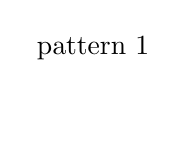
\begin{tikzpicture}
\node [] (n0)  at (0.0,0.0) {};
\node [] (n1)  at (0.0,1.0) {pattern 1}; 
\end{tikzpicture} 
&
\begin{tikzpicture}
\node [] (n1)  at (0.0,2.0) {$T_1 \rightarrow R_1$}; 
\node [] (n2)  at (1.8,1.0) {$T_2 (= R_1) \rightarrow R_3$};
\node [] (n3)  at (4.2,0.0) {$T_3 (= R_2) \rightarrow R_4$}; 

\draw[->] (0.5,1.7) -- (0.5,1.3);
\draw[->] (3.0,0.7) -- (3.0,0.3);


\end{tikzpicture}

\\\hline

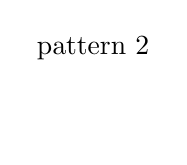
\begin{tikzpicture}
\node [] (n0)  at (0.0,0.0) {};
\node [] (n1)  at (0.0,1.0) {pattern 2}; 
\end{tikzpicture} 
 &
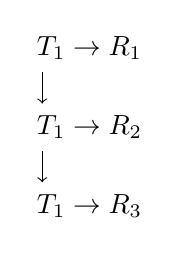
\begin{tikzpicture}
\node [] (n1)  at (0.0,2.0) {$T_1 \rightarrow R_1$}; 
\node [] (n2)  at (0.0,1.0) {$T_1 \rightarrow R_2$};
\node [] (n3)  at (0.0,0.0) {$T_1 \rightarrow R_3$}; 

\draw[->] (-0.6,1.7) -- (-0.6,1.3);
\draw[->] (-0.6,0.7) -- (-0.6,0.3);
\end{tikzpicture}

\\\hline
\begin{tikzpicture}
\node [] (n0)  at (0.0,0.0) {};
\node [] (n1)  at (0.0,2.0) {pattern 3}; 
\end{tikzpicture} 
&
\begin{tikzpicture}
\node [] (n0)  at (2.2,4.0) {$[T]$}; 
\node [] (n1)  at (0.0,3.0) {$T_1 \rightarrow R_1$}; 
\node [] (n2)  at (1.8,2.0) {$T_2 \rightarrow R_2$};
\node [] (n3)  at (4.2,1.0) {$T_3  \rightarrow R_3$}; 

\draw[->] (n0.south) -- (-0.5,3.3);
\draw[->] (n0.south) -- (1.3,2.3);
\draw[->] (n0.south) -- (3.5,1.3);
\end{tikzpicture}

\\\hline

\begin{tikzpicture}
\node [] (n0)  at (0.0,0.0) {};
\node [] (n1)  at (0.0,2.0) {pattern 4}; 
\end{tikzpicture} 
&
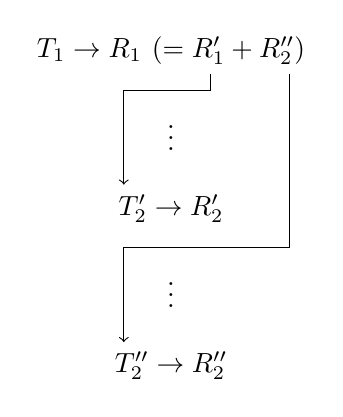
\begin{tikzpicture}
\node [] (n0)  at (0.0,4.0) {$T_1 \rightarrow R_1\textit{ }( = R_1^\prime + R_2^{\prime\prime} )$}; 

\node [] (d0)  at (0.0,3) {$\vdots$}; 

\node [] (n1)  at (0.0,2) {$T_2^\prime \rightarrow R_2^\prime$}; 


\node [] (d0)  at (0.0,1) {$\vdots$}; 


\node [] (n2)  at (0.0,0.0) {$T_2^{\prime\prime} \rightarrow R_2^{\prime\prime}$};

\draw [->] (0.5, 3.7) -- (0.5, 3.5) -- (-0.6, 3.5) -- (-0.6, 2.3);

\draw [->] (1.5, 3.7) -- (1.5, 1.5) -- (-0.6, 1.5) -- (-0.6, 0.3);

\end{tikzpicture}

\end{tabular}
\caption{In the notation used by (?), the horizontal arrow indicates a transition in an utterance, while the vertical one indicates the the contextual connection within of utterances.}
\label{Table:danesh_coherence_patterns}
\end{table}


\newcite{danes74a} interprets the patterns as follows:

\begin{itemize}
\item Pattern 1: A linear transition pattern between themes and rhymes. 
In this pattern, each utterance takes the rhyme presented in the preceding context of the utterance as a given information and transfers it to a new information or a new rhyme. 
In other words, each R (i.e. a new information) becomes the T (i.e. a given information) of the next utterance. 


\item Pattern 2: This pattern depicts a constant theme that continues across utterances. 
One and the same theme appears in a series of utterances. 
Each utterance, however, presents new information about the theme. 


\item Pattern 3: In this pattern $[T]$ indicates a hypertheme that is a global theme of a paragraph or even other text sections. 
 Pattern shows that different utterances can be connected because the themes, or the given information,  of utterances are semantically connected to a hypertheme. 

 \item Pattern 4: 
 \newcite{danes74a} expresses that different combination of these patterns can be employed in different texts. 
 Some of such combinations are so frequent that can be taken as special type of theme-rhyme transition of a higher order. 
  \newcite{danes74a} finds Pattern 4 as one of the most important of such patterns, where an utterance presents two (which can in potential several) rhymes, $R^\prime$ and $R^{\prime\prime}$ , in connection with a given theme. 
  First $R^{\prime}$ expounded and after its progression has been finished, $R^{\prime\prime}$ becomes the theme of another transition. 
  Transitions in between for extending each rhyme follows its own pattern. 
\end{itemize}

\newcite{danes74a} brings this point into attention that one of the important properties of these patterns is omitting links in these patterns.  
For example, in Pattern 1 there is no link between the earliest and latest utterance. 
Those are connected because there is an intermediate utterance that makes transitions between themes and rhymes smoother. 
In contrast, all utterances in Pattern 3  are linked to each other because they all have $T_1$ as a shared given information. 

What \newcite{danes74a} proposed is that the generalized structure of coherent texts may be described in terms of an underlying patterns of transitions between presented themes and rhymes.
This theory is the main motivation of our coherence model in this chapter. 
As before we take entities mentioned in a text as piece of information that make sentences connected. 
The entity graph representation, introduced in Chapter \ref{}, is employed to model the distribution of entities across sentences of a text. 
Then the projection graphs obtained from the entity graph representations of texts model the general structure of sentence node connectivity of texts. 
The entity graph model uses the average ourdegree to encode the connectivity of sentence nodes in projection graphs. 

The main research questions that are investigated in this chapter is:

\begin{itemize}
% \item Is the average outdegree proposed by \newcite{guinaudeau13}  a strong representative metric for the connectivity style of projection graphs and therefore the perceived coherence of texts?
\item Are the any more representative features for the connectivity style of nodes in projection graphs?
\end{itemize}

The idea is to check how well the average outdegree metric models the coherence of a set of well-written articles such as published news articles in Wall Street Journal corpus.  
In spite of this fact that these articles are written by professional authors, human judges assigned to them different range of readability scores (More details in Section \ref{}).  
% We compute the Pearson correlation between the average outdegree of projection graph representations of news articles and their associated score assigned by human judges. 

In order to answer the research question, we employ a subgraph mining algorithm to automatically extract all  subgraphs occurring in projection graphs of these news articles. 
Automatically extracting subgraphs of projection graphs in order to model coherence is our novel contribution in this chapter. 
However, we show that there is a similarity between the automatically mined subgraphs of projection graphs and the coherence patterns proposed by \newcite{danes74a}, indicating that our model's foundation is also linguistically sound.  

We define the frequency of these systematic extracted subgraphs (or coherence patterns) as features that capture the connectivity style of nodes in a projection graph and therefore the coherence property of the corresponding text.  
We evaluate if our novel coherence features outperform the average outdegree feature in a classification task in that more coherent texts should be recognized from less coherent texts. 
In next section, we explain how we exactly model coherence patterns. 


\section{Definitions From Graph Theory}
\label{sec:definition_from_graph_theory}
%
In order to explain the applied subgraphs that encode coherence of sentences in a text, we first need to define some required concepts from graph theory. 

\textbf{Graph.}
A graph is a set of points, we refer to them as nodes, connected by lines, called edges. 
More formally, a graph is a pair of two finite sets $G=( V, E )$ where $V$ is a set of nodes and $E$ is a set of edges whose elements are pairs of nodes. 

\begin{figure}[!ht]
\centering
\small
\begin{tabular}{cc}

	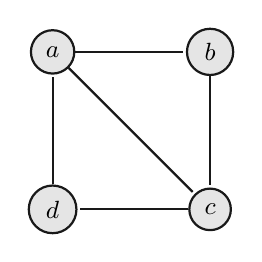
\begin{tikzpicture}[shorten >=1pt,-,scale=0.5]  
		\tikzstyle{node}=[circle,thick,draw=black!90,fill=black!10,minimum size=2mm]
		\tikzstyle{edge}=[draw=black!90, thick]
	   
		 \node [node] (a) at (0,4) {\small{$a$}};
		 \node [node] (b) at (4,4) {\small{$b$}};
		 \node [node] (d) at (0,0) {\small{$d$}}; 
		 \node [node] (c) at (4,0) {\small{$c$}}; 
		 
		 \path[edge] (a) -- (b);
		 \path[edge] (b) -- (c);
		 \path[edge] (c) -- (d);
		 \path[edge] (d) -- (a);
		 \path[edge] (a) -- (c);
       
	\end{tikzpicture}

	&

	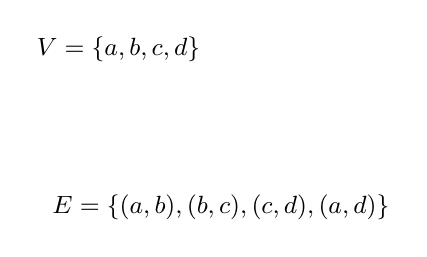
\begin{tikzpicture}[shorten >=1pt,-,scale=0.5]  

		 \node (a) at (0,4) {\small{$V = \left \{ a,b,c,d \right \}$}};
		 \node (b) at (2.6,0) {\small{$E = \left \{(a,b),(b,c),(c,d),(a,d) \right \} $}};

	\end{tikzpicture}

	\\

	$G$ 
	&
	$V:Nodes,E:Edges$ 

\end{tabular}
\caption{Graph. }
\label{fig:graph}
\end{figure} 

If the direction of edges conveys any meaning, then edges can be directed so that for any edge like $e = (x,y)$ the direction is from $x$ towards $y$, which are respectively called the source node and the end node of edge $e$. 
Figure \ref{fig:dir_graph} shows the directed version of the shown graph in Figure \ref{fig:graph}.

\begin{figure}[!ht]
\centering
\small
\begin{tabular}{c}

	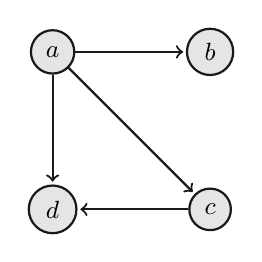
\begin{tikzpicture}[shorten >=1pt,-,scale=0.5]  
		\tikzstyle{node}=[circle,thick,draw=black!90,fill=black!10,minimum size=2mm]
		\tikzstyle{edge}=[draw=black!90, thick]
	   
		 \node [node] (a) at (0,4) {\small{$a$}};
		 \node [node] (b) at (4,4) {\small{$b$}};
		 \node [node] (d) at (0,0) {\small{$d$}}; 
		 \node [node] (c) at (4,0) {\small{$c$}}; 
		 
		 \path[edge,->] (a) -- (b);
		 %\path[edge,->] (b) -- (c);
		 \path[edge,->] (c) -- (d);
		 \path[edge,->] (a) -- (d);
		 \path[edge,->] (a) -- (c);
       
	\end{tikzpicture}
\\

	$G$ 

\end{tabular}
\caption{Directed graph of graph $G$ in Figure \ref{fig:graph}. }
\label{fig:dir_graph}
\end{figure} 


\textbf{Isomorphic.} 
%
Two graphs $G_1$ and $G_2$ are isomorphic, if they fulfill two conditions: (i) a one\--to\--one association, like $f$, exists between nodes of $G_1$ and those of $G_2$, and two nodes of $G_2$ should be connected, if and only if their associated nodes in $G_1$ are connected. 
Figure \ref{fig:isomorphic_graph} illustrates two isomorphic graphs. 
More formally, an isomorphism of graph $G_1$ and $G_2$ is an association between node sets of these graphs:

\begin{equation}
f: V \left( G_1 \right) \rightarrow V \left( G_2 \right),
\end{equation}

such that any  two nodes $u$ and $v$ of $G_1$ are adjacent in $G_1$ if and only if $f \left( u \right)$ and $f \left( v \right)$ are adjacent in $G_2$.
If an isomorphism exists between two graphs, then the graphs are called isomorphic.

\begin{figure}[!ht]
\centering
\small
\begin{tabular}{c@{\hskip 2.5cm}c@{\hskip 2.5cm}c}

	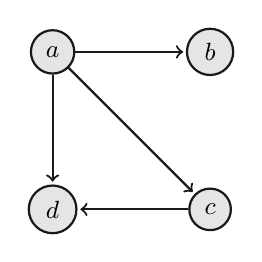
\begin{tikzpicture}[shorten >=1pt,-,scale=0.5]  
		\tikzstyle{node}=[circle,thick,draw=black!90,fill=black!10,minimum size=2mm]
		\tikzstyle{edge}=[draw=black!90, thick]
	   
		 \node [node] (a) at (0,4) {\small{$a$}};
		 \node [node] (b) at (4,4) {\small{$b$}};
		 \node [node] (d) at (0,0) {\small{$d$}}; 
		 \node [node] (c) at (4,0) {\small{$c$}}; 
		 
		 \path[edge,->] (a) -- (b);
		 %\path[edge,->] (b) -- (c);
		 \path[edge,->] (a) -- (c);
		 \path[edge,->] (c) -- (d);
		 \path[edge,->] (a) -- (d);
       
	\end{tikzpicture}

	 &

  	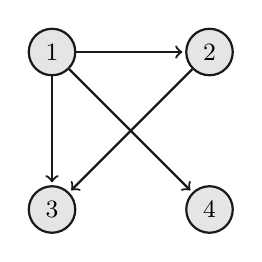
\begin{tikzpicture}[shorten >=1pt,-,scale=0.5]  
	\tikzstyle{node}=[circle,thick,draw=black!90,fill=black!10,minimum size=2mm]
	\tikzstyle{edge}=[draw=black!90, thick]
   
	 \node [node] (1) at (0,4) {\small{$1$}};
	 \node [node] (2) at (4,4) {\small{$2$}};
	 \node [node] (3) at (4,0) {\small{$4$}}; 
	 \node [node] (4) at (0,0) {\small{$3$}}; 
	 
	 \path[edge,->] (1) -- (2);
	 \path[edge,->] (1) -- (3);
	 \path[edge,->] (1) -- (4);
	 \path[edge,->] (2) -- (4);
   
  \end{tikzpicture}

	 &

  	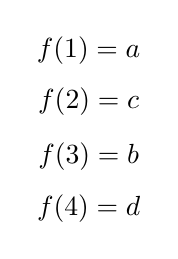
\begin{tikzpicture}[shorten >=1pt,-,scale=0.5]  

	 \node  (1) at (0,4) {$f(1) = a$};
	 \node  (2) at (0,2.7) {$f(2) = c$};
	 \node  (3) at (0,1.3) {$f(3) = b$}; 
	 \node  (4) at (0,0) {$f(4) = d$}; 

  \end{tikzpicture}
\\
$ G_1 $ 
&
 $G_2$
& 
$\textit{Node associations}$

\end{tabular}
\caption{Two isomorphic graphs and a sample association between their nodes. }
\label{fig:isomorphic_graph}
\end{figure} 


\textbf{Subgraph.} 
%
Graph $G_2$ is a subgraph of graph $G_1$, if $G_2$ is isomorphic to a graph whose nodes and edges are a subset of nodes and edges of $G_1$.
\begin{figure}[!ht]
\centering
\small
\begin{tabular}{c@{\hskip 2.5cm}c@{\hskip 2.5cm}c}

	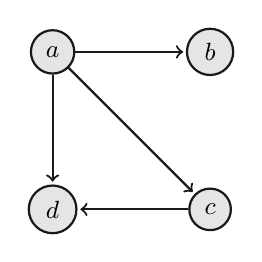
\begin{tikzpicture}[shorten >=1pt,-,scale=0.5]  
		\tikzstyle{node}=[circle,thick,draw=black!90,fill=black!10,minimum size=2mm]
		\tikzstyle{edge}=[draw=black!90, thick]
	   
		 \node [node] (a) at (0,4) {\small{$a$}};
		 \node [node] (b) at (4,4) {\small{$b$}};
		 \node [node] (d) at (0,0) {\small{$d$}}; 
		 \node [node] (c) at (4,0) {\small{$c$}}; 
		 
		 \path[edge,->] (a) -- (b);
		 %\path[edge,->] (b) -- (c);
		 \path[edge,->] (a) -- (c);
		 \path[edge,->] (c) -- (d);
		 \path[edge,->] (a) -- (d);

       
	\end{tikzpicture}

	 &

  	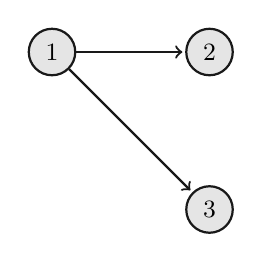
\begin{tikzpicture}[shorten >=1pt,-,scale=0.5]  
	\tikzstyle{node}=[circle,thick,draw=black!90,fill=black!10,minimum size=2mm]
	\tikzstyle{edge}=[draw=black!90, thick]
   
	 \node [node] (1) at (0,4) {\small{$1$}};
	 \node [node] (2) at (4,4) {\small{$2$}};
	 \node [node] (3) at (4,0) {\small{$3$}}; 
	 
	 \path[edge,->] (1) -- (2);
	 \path[edge,->] (1) -- (3);
   
  \end{tikzpicture}

	 &

  	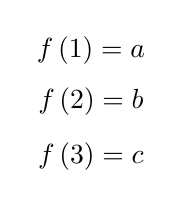
\begin{tikzpicture}[shorten >=1pt,-,scale=0.5]  

	 \node  (1) at (0,4) {$f \left( 1 \right) = a$};
	 \node  (2) at (0,2.7) {$f \left( 2 \right) = b$};
	 \node  (3) at (0,1.3) {$f \left( 3 \right) = c$}; 

  \end{tikzpicture}
\\
$ G_1 $ & $G_2$  & $\textit{Node associations}$

\end{tabular}
\caption{$G_2$ is a subgraphs of graph $G_1$}
\label{fig:subgraph}
\end{figure} 

In the shown example in Figure \ref{fig:subgraph}, graph $G_2$ is isomorphic with graph 

\begin{equation}
G = \left( \left\{ a,b,c \right\}, \left\{ \left( a , b \right),\left( b , c \right) \right\} \right) 
\end{equation}

whose node and edge sets are subsets of node and edge sets of $G_1$.

\textbf{k-node subgraph.}
%
The size of subgraph is the size of its node set that is the number nodes in the graph. 
Graph $G_2 = \left( V_2 , E_2 \right)$ is a k-node subgraph of graph $G_1 = \left( V_1, E_1 \right)$, if $G_2$ is a subgraph of $G_1$, and $V_2$ has $k$ elements, $|V_2|=k$. 
In Figure \ref{fig:subgraph}, graph $G_2$ is a 3-node subgraph of graph $G_1$. 


\textbf{Induced subgraph.} 
%
An induced subgraph of a graph is a subgraph of the graph with an extra condition on its edges.  
That is, in simple words, its edge sets contains all possible edges that are present in the main graph. 
Formally, graph $G_2 = (V_2, E_2)$ is an induced subgraph of graph $G_1 = (V_2, E_2)$ if $V_2 \subseteq V_1$ and 
\begin{equation}
E_2 = \left\{ (x,y)| x \in V_2, y \in V_2, (x,y) \in E_1   \right\}. 
\end{equation}

Figure \ref{fig:induced_subgraphs} shows a graph and two subgraphs of it. 
Subgraph $G_2$ is a subgraph of $G_1$ but not induced, because there is no edge between nodes $1$ and $3$ of this subgraph while their associated nodes, $a$ and $b$, in graph $G_1$ are connected. 
In contrast, subgraph $G_2$ is an induced subgraph of $G_1$ because it contains all possible edges that are present in $G_1$ and connect nodes of the subgraph.  

\begin{figure}[!ht]
\centering
\small
\begin{tabular}{c@{\hskip 1.5cm}c@{\hskip 1.5cm}c@{\hskip 1.5cm}c}

	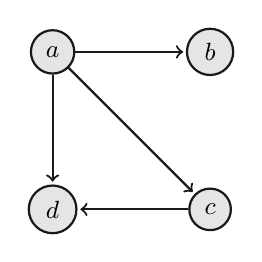
\begin{tikzpicture}[shorten >=1pt,-,scale=0.5]  
		\tikzstyle{node}=[circle,thick,draw=black!90,fill=black!10,minimum size=2mm]
		\tikzstyle{edge}=[draw=black!90, thick]
	   
		 \node [node] (a) at (0,4) {\small{$a$}};
		 \node [node] (b) at (4,4) {\small{$b$}};
		 \node [node] (d) at (0,0) {\small{$d$}}; 
		 \node [node] (c) at (4,0) {\small{$c$}}; 
		 
		 \path[edge,->] (a) -- (b);
		 \path[edge,->] (a) -- (c);
		 \path[edge,->] (c) -- (d);
		 \path[edge,->] (a) -- (d);

       
	\end{tikzpicture}

	 &

  	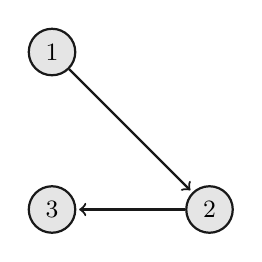
\begin{tikzpicture}[shorten >=1pt,-,scale=0.5]  
	\tikzstyle{node}=[circle,thick,draw=black!90,fill=black!10,minimum size=2mm]
	\tikzstyle{edge}=[draw=black!90, thick]
   
	 \node [node] (1) at (0,4) {\small{$1$}};
	 \node [node] (2) at (4,0) {\small{$2$}};
	 \node [node] (3) at (0,0) {\small{$3$}}; 
	 
	 \path[edge,->] (1) -- (2);
	 \path[edge,->] (2) -- (3);
   
  \end{tikzpicture}

	 &


  	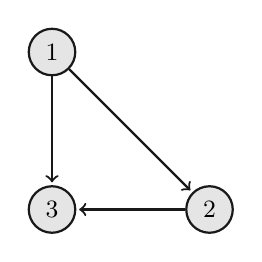
\begin{tikzpicture}[shorten >=1pt,-,scale=0.5]  
	\tikzstyle{node}=[circle,thick,draw=black!90,fill=black!10,minimum size=2mm]
	\tikzstyle{edge}=[draw=black!90, thick]
   
	 \node [node] (1) at (0,4) {\small{$1$}};
	 \node [node] (2) at (4,0) {\small{$2$}};
	 \node [node] (3) at (0,0) {\small{$3$}}; 
	 
	 \path[edge,->] (1) -- (2);
	 \path[edge,->] (2) -- (3);
	 \path[edge,->] (1) -- (3);
   
  \end{tikzpicture}

  &

  	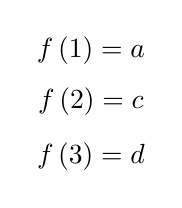
\begin{tikzpicture}[shorten >=1pt,-,scale=0.5]  

	 \node  (1) at (0,4) {$f \left( 1 \right) = a$};
	 \node  (2) at (0,2.7) {$f \left( 2 \right) = c$};
	 \node  (3) at (0,1.3) {$f \left( 3 \right) = d$}; 

  \end{tikzpicture}
\\
$ G_1 $ & $G_2$  & $G_3$ & $\textit{Node associations}$

\end{tabular}
\caption{Induced subgraphs}
\label{fig:induced_subgraphs}
\end{figure} 

It is worth mentioning that henceforth we mean induced subgraphs when using the term subgraph.  
However, in cases that the context is not clear we explicitly distinguish them.     


\textbf{Graph signature.} 
%
Given a list of graphs $ \zeta  = \left[ G_1, G_2, \cdots , G_m \right]$,  a graph signature, which is  denoted by for graph $G$, denoted by $\phi \left( G \right)$,  with respect to $\zeta$ is a vector of frequencies of graphs in $\zeta$ in graph $G$:

\begin{equation}
\phi \left( G \right) = \left( f_1, f_2, f_3, \cdots, f_m \right),
\end{equation}
%
where $f_i$ is the frequency of graphs in graph $G$. 
The frequency of graph $G_i$ in graph $G$ is computed as follows:

\begin{equation}
 f_i = \frac{count(G_i, G)}{\sum_{G_j \in \zeta}{count(G_j, G)}}
\end{equation}
%
where $count(G_i, G)$ is the number of occurrences of $G_i$ in graph $G$. 
The reason of using frequency instead of raw count is that frequency is a normalized value that cannot become biased to the number of nodes and edges of graph $G$. 



\section{Coherence Patterns Modeling}
\label{sec:coherence_patterns_modeling}
%
The entity graph representation of a text encodes the distribution of entities across sentences of a text. 
One-mode projection graphs model the connectivity between sentence nodes with respect to the shared entities between sentences. 
Our main contribution, in this chapter, is that instead of the average outdegree as a simple metric that models the connectivity of sentence nodes of a projection graph, we introduce a set of novel graph-based features that encode the structure of connections (i.e.\ connectivity style) in a projection graph. 
We hypothesize that the frequencies of different subgraphs occurring in projection graphs encode the connectivity style of  projection graphs and therefore, they can be utilized to model coherence.  
Our experiments in Section \ref{} indicate this hypothesis is correct for the examined tasks.  

Given a corpus of documents, we model connections between sentences of each document by its projection graph representation, $P_U$. 
In this step, instead of having a set of documents we have a set of one-mode projection graphs associated with documents. 
We refer to it as the graph set.  
Similar to the entity grid model \cite{barzilay08b}, the key assumption behind our coherence model is that coherent texts reveal similar patterns that differ them from incoherent texts. 
Therefore, the projection graphs of coherent texts reveal similar connectivity style that is different with incoherent texts. 
\newcite{guinaudu13} propose the average outdegree, but we propose to use the graph signature of each projection graph to encode the connectivity style of projection graphs into a vector. 

In order to obtain graph signatures of projection graphs, some basis graphs are required to represent projection graphs based on them. 
We propose to extract all possible subgraphs of projection graphs as basis graphs for computing graph signatures. 

The results of our experiments in Section \ref{}, show that the frequencies of some subgraphs in documents are statistically significantly correlated with scores assigned by human annotators to documents. 
Moreover, as it will be shown in Section \ref{}, some of these subgraphs are similar to what are defined by \newcite{danes74a}. 
Considering these all, we refer to these subgraphs coherence patterns and their frequencies as coherence features.  

Figure \ref{} shows a schema of our idea for extracting coherence patterns and features. 

From the machine learning perspective, the vector representation of the projection graphs can be taken as feature vectors, in which each element is a feature representing one aspect of data. 
These feature vectors can be supplied for training any machine learning model in order to classify coherent documents from incoherent documents. 

\subsection{Subgraph Mining}
\label{subsec:subgraph_mining}
%
Coherence patterns are subgraphs that occur at least in one of projection graphs of documents in a corpus. 
Mining all subgraphs that occur in a graph set is computationally expensive and this problem is proved to be an NP-complete problem \cite{}. 
Intuitively, a graph with $\Vert E \Vert$ edges, potentially has $\mathcal{O} \left( 2^{\Vert E \Vert} \right)$ subgraphs.  
Projection graphs with $\Vert V \Vert$ nodes at most has  $\frac{(n-1)(n-2)}{2}$ that is in order of $\mathcal{O} \left( \Vert V \Vert \right)$.  

In general, the goal of this thesis is not to develop an algorithm for subgraph mining. 
This has been widely studied in computer science and different algorithms and packages have been developed for this. 
The gSpan\footnote{We use the Java package: \url{http://www.cs.ucsb.edu/~xyan/software/gSpan.htm}}  algorithm \cite{yanxifeng02} is one of the efficient methods for mining subgraphs of a  graph set. 
Here, we briefly describe the idea and the method of the gSpan algorithm and refer interested readers to Appendix \ref{} for more details. 

The gSpan,(\textit{g}raph-based \textit{S}ubstructure \textit{pa}ttern \textit{m}ining), algorithm is an approach for extracting all patterns (i.e. subgraphs) that frequently occur in a graph set. 
It discovers all frequent subgraphs without generating the candidates. 
So it is more efficient. 
A subgraph is called frequent if the number of graphs that contain the subgraph is greater than a threshold. 
This threshold is a hyper-parameter of the algorithm\footnote{We always set this threshold to zero to extract all occurring subgraphs in a graph set. We prefer all patterns over frequent patterns because our goal is to investigate .....
 However, is it possible to integrate this in the future work?}.
 gSpan orders graphs in a graph set with respect to their structures and then adapts a depth-first-search search strategy to extract frequent connected subgraphs efficiently. 
 It starts with small subgraphs and simultaneously expands subgraphs and check the frequency of subgraph. 

 [It seems the efficiency of gSpan is when you have a threshold, by setting this to zero it has to extract all possible patterns, so the method is still expensive..]









Subgraph features are divided into two categories: basic subgraphs and frequent large subgraphs.

\textbf{Basic subgraphs.} Instead of frequent subgraphs all possible 3-node subgraphs (Figure \ref{f:all_3node_subgraphs}) are used as
basic subgraphs because they are the smallest meaningful subgraphs that can model coherence patterns. 

Because backward edges never occur in one-mode projections, only four subgraphs are feasible (Figure \ref{f:feasible_3node_subgraphs}).

%\begin{figure}[!ht]
\centering
\resizebox{1.0\columnwidth}{!}{
\begin{tabular}{cccc}
 %%%%%%%%%%%%%%%%%%%%%%%%%%%%%% subgraph 1 %%%%%%%%%%%%%%%%%%%%%%%%%%%%%%
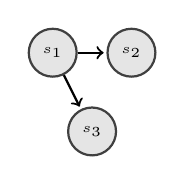
\begin{tikzpicture}[shorten >=1pt,->,scale=0.5]  
        \tikzstyle{sentence}=[circle,thick,draw=black!75,fill=black!10,minimum size=2mm]
        \tikzstyle{edge}=[draw, thick]
       \begin{scope}
         \node [sentence] (s1) at (0,2) {\tiny{$s_1$}};
         \node [sentence] (s2) at (2,2) {\tiny{$s_2$}};
         \node [sentence] (s3) at (1,0) {\tiny{$s_3$}}; 
         \path[edge] (s1) edge [above] node[font=\tiny] {} (s2);
         \path[edge] (s1) edge [above] node[font=\tiny] {} (s3);
        \end{scope}        
      \end{tikzpicture}
&
%%%%%%%%%%%%%%%%%%%%%%%%%%%%%% subgraph 2 %%%%%%%%%%%%%%%%%%%%%%%%%%%%%%
 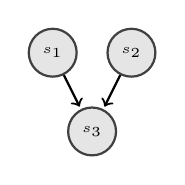
\begin{tikzpicture}[shorten >=1pt,->,scale=0.5]  
        \tikzstyle{sentence}=[circle,thick,draw=black!75,fill=black!10,minimum size=2mm]
        \tikzstyle{edge}=[draw, thick]
       \begin{scope}
         \node [sentence] (s1) at (0,2) {\tiny{$s_1$}};
         \node [sentence] (s2) at (2,2) {\tiny{$s_2$}};
         \node [sentence] (s3) at (1,0) {\tiny{$s_3$}}; 
         \path[edge] (s1) edge [above] node[font=\tiny] {} (s3);
         \path[edge] (s2) edge [above] node[font=\tiny] {} (s3);
        \end{scope}        
      \end{tikzpicture}

&
 %%%%%%%%%%%%%%%%%%%%%%%%%%%%%% subgraph 3 %%%%%%%%%%%%%%%%%%%%%%%%%%%%%%
 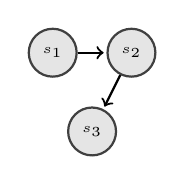
\begin{tikzpicture}[shorten >=1pt,->,scale=0.5]  
        \tikzstyle{sentence}=[circle,thick,draw=black!75,fill=black!10,minimum size=2mm]
        \tikzstyle{edge}=[draw, thick]
       \begin{scope}
         \node [sentence] (s1) at (0,2) {\tiny{$s_1$}};
         \node [sentence] (s2) at (2,2) {\tiny{$s_2$}};
         \node [sentence] (s3) at (1,0) {\tiny{$s_3$}}; 
         \path[edge] (s1) edge [above] node[font=\tiny] {} (s2);
         \path[edge] (s2) edge [above] node[font=\tiny] {} (s3);
        \end{scope}        
      \end{tikzpicture}
      
      
 &
 %%%%%%%%%%%%%%%%%%%%%%%%%%%%%% subgraph 7 %%%%%%%%%%%%%%%%%%%%%%%%%%%%%%
 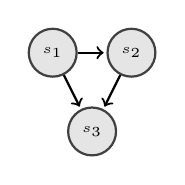
\begin{tikzpicture}[shorten >=1pt,->,scale=0.5]  
        \tikzstyle{sentence}=[circle,thick,draw=black!75,fill=black!10,minimum size=2mm]
        \tikzstyle{edge}=[draw, thick]
       \begin{scope}
        \node [sentence] (s1) at (0,2) {\tiny{$s_1$}};
         \node [sentence] (s2) at (2,2) {\tiny{$s_2$}};
         \node [sentence] (s3) at (1,0) {\tiny{$s_3$}}; 

         
         \path[edge] (s1) edge [above] node[font=\tiny] {} (s2);
         \path[edge] (s1) edge [above] node[font=\tiny] {} (s3);
         \path[edge] (s2) edge [above] node[font=\tiny] {} (s3);
         
        \end{scope}        
      \end{tikzpicture} 
\\

\scriptsize{$sg_1$} & \scriptsize{$sg_2$} & \scriptsize{$sg_3$}& \scriptsize{$sg_4$}
                 

\end{tabular}
}
\caption{Feasible 3\--node subgraph coherence features.}
\label{f:feasible_3node_subgraphs}
\end{figure}

We interpret these subgraphs as follows:

\begin{itemize}
\item \boldmath{$sg_1$}: The connection between a sentence and subsequent ones. In other words, at least two entities are mentioned in one sentence and the subsequent ones are about these entities.

\item \boldmath{$sg_2$}: Indicates that entities in $s_t$ and $s_u$ get connected to each other in $s_v$.

\item \boldmath{$sg_3$}: Each sentence tends to refer to the most prominent entity (focus of attention) in preceding sentences \cite{sidner83,grosz95}. 
The absence of a connection between $s_t$ and $s_v$ indicates that the entity connecting $s_t$ and $s_u$ is different from the entity connecting $s_u$ and $s_v$. 
Therefore this subgraph approximately corresponds to the shift of the focus of attention.

\item \boldmath{$sg_4$}: Merges $sg_1$ and $sg_3$ and represents all connections of these two subgraphs.
\end{itemize}

We use these feasible 3-node subgraphs and compute the graph signature, $\Phi$, of each $G\in\zeta$. 
We propose each $\varphi\in\Phi$ (i.e. relative frequency of each subgraph in $G$) as a connectivity feature of graph $G$ to measure text coherence. 

%\begin{figure}[!ht]
\centering
\small
\resizebox{1.0\columnwidth}{!}{
\begin{tabular}{cccccccc}
 %%%%%%%%%%%%%%%%%%%%%%%%%%%%%% subgraph 1 %%%%%%%%%%%%%%%%%%%%%%%%%%%%%%
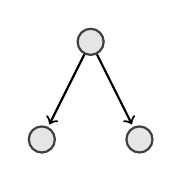
\begin{tikzpicture}[shorten >=1pt,->,scale=0.62]  
        \tikzstyle{sentence}=[circle,thick,draw=black!75,fill=black!10,minimum size=2mm]
        \tikzstyle{edge}=[draw, thick]
       \begin{scope}
         \node [sentence] (s1) at (1,2) {\tiny{}};
         \node [sentence] (s2) at (0,0) {\tiny{}};
         \node [sentence] (s3) at (2,0) {\tiny{}}; 
         \path[edge] (s1) edge [above] node[font=\tiny] {} (s2);
         \path[edge] (s1) edge [above] node[font=\tiny] {} (s3);
        \end{scope}        
      \end{tikzpicture}
&
 %%%%%%%%%%%%%%%%%%%%%%%%%%%%%% subgraph 2 %%%%%%%%%%%%%%%%%%%%%%%%%%%%%%
 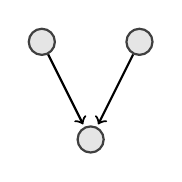
\begin{tikzpicture}[shorten >=1pt,->,scale=0.62]  
        \tikzstyle{sentence}=[circle,thick,draw=black!75,fill=black!10,minimum size=2mm]
        \tikzstyle{edge}=[draw, thick]
       \begin{scope}
         \node [sentence] (s1) at (0,2) {\tiny{}};
         \node [sentence] (s2) at (2,2) {\tiny{}};
         \node [sentence] (s3) at (1,0) {\tiny{}}; 
         \path[edge] (s1) edge [above] node[font=\tiny] {} (s3);
         \path[edge] (s2) edge [above] node[font=\tiny] {} (s3);
        \end{scope}        
      \end{tikzpicture}

&
 %%%%%%%%%%%%%%%%%%%%%%%%%%%%%% subgraph 3 %%%%%%%%%%%%%%%%%%%%%%%%%%%%%%
 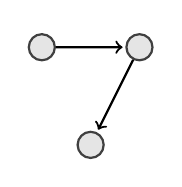
\begin{tikzpicture}[shorten >=1pt,->,scale=0.62]  
        \tikzstyle{sentence}=[circle,thick,draw=black!75,fill=black!10,minimum size=2mm]
        \tikzstyle{edge}=[draw, thick]
       \begin{scope}
         \node [sentence] (s1) at (0,2) {\tiny{}};
         \node [sentence] (s2) at (2,2) {\tiny{}};
         \node [sentence] (s3) at (1,0) {\tiny{}}; 
         \path[edge] (s1) edge [above] node[font=\tiny] {} (s2);
         \path[edge] (s2) edge [above] node[font=\tiny] {} (s3);
        \end{scope}        
      \end{tikzpicture}
      
&
 %%%%%%%%%%%%%%%%%%%%%%%%%%%%%% subgraph 4 %%%%%%%%%%%%%%%%%%%%%%%%%%%%%%
 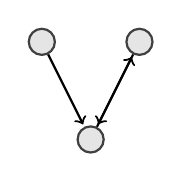
\begin{tikzpicture}[shorten >=1pt,->,scale=0.62]  
        \tikzstyle{sentence}=[circle,thick,draw=black!75,fill=black!10,minimum size=2mm]
        \tikzstyle{edge}=[draw, thick]
       \begin{scope}
         \node [sentence] (s1) at (0,2) {\tiny{}};
         \node [sentence] (s2) at (2,2) {\tiny{}};
         \node [sentence] (s3) at (1,0) {\tiny{}}; 
         \path[edge] (s1) edge [above] node[font=\tiny] {} (s3);
         \path[edge] (s2) edge [above] node[font=\tiny] {} (s3);
         \path[edge] (s3) edge [above] node[font=\tiny] {} (s2);
         
        \end{scope}        
      \end{tikzpicture}      
      
&
 %%%%%%%%%%%%%%%%%%%%%%%%%%%%%% subgraph 5 %%%%%%%%%%%%%%%%%%%%%%%%%%%%%%
 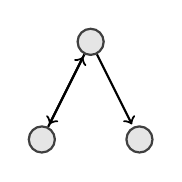
\begin{tikzpicture}[shorten >=1pt,->,scale=0.62]  
        \tikzstyle{sentence}=[circle,thick,draw=black!75,fill=black!10,minimum size=2mm]
        \tikzstyle{edge}=[draw, thick]
       \begin{scope}
         \node [sentence] (s1) at (1,2) {\tiny{}};
         \node [sentence] (s2) at (0,0) {\tiny{}};
         \node [sentence] (s3) at (2,0) {\tiny{}}; 
         \path[edge] (s2) edge [above] node[font=\tiny] {} (s1);
         \path[edge] (s1) edge [above] node[font=\tiny] {} (s2);
         \path[edge] (s1) edge [above] node[font=\tiny] {} (s3);
         
        \end{scope}        
      \end{tikzpicture}            
      
 &
 %%%%%%%%%%%%%%%%%%%%%%%%%%%%%% subgraph 6 %%%%%%%%%%%%%%%%%%%%%%%%%%%%%%
 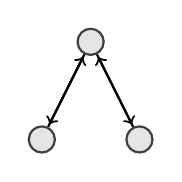
\begin{tikzpicture}[shorten >=1pt,->,scale=0.62]  
        \tikzstyle{sentence}=[circle,thick,draw=black!75,fill=black!10,minimum size=2mm]
        \tikzstyle{edge}=[draw, thick]
       \begin{scope}
         \node [sentence] (s1) at (1,2) {\tiny{}};
         \node [sentence] (s2) at (0,0) {\tiny{}};
         \node [sentence] (s3) at (2,0) {\tiny{}}; 
         \path[edge] (s2) edge [above] node[font=\tiny] {} (s1);
         \path[edge] (s1) edge [above] node[font=\tiny] {} (s2);
         \path[edge] (s1) edge [above] node[font=\tiny] {} (s3);
         \path[edge] (s3) edge [above] node[font=\tiny] {} (s1);
         
        \end{scope}        
      \end{tikzpicture}            
      
 &
 %%%%%%%%%%%%%%%%%%%%%%%%%%%%%% subgraph 7 %%%%%%%%%%%%%%%%%%%%%%%%%%%%%%
 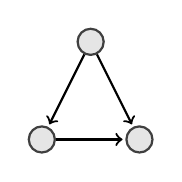
\begin{tikzpicture}[shorten >=1pt,->,scale=0.62]  
        \tikzstyle{sentence}=[circle,thick,draw=black!75,fill=black!10,minimum size=2mm]
        \tikzstyle{edge}=[draw, thick]
       \begin{scope}
         \node [sentence] (s1) at (1,2) {\tiny{}};
         \node [sentence] (s2) at (0,0) {\tiny{}};
         \node [sentence] (s3) at (2,0) {\tiny{}}; 
         
         \path[edge] (s1) edge [above] node[font=\tiny] {} (s2);
         \path[edge] (s1) edge [above] node[font=\tiny] {} (s3);
         \path[edge] (s2) edge [above] node[font=\tiny] {} (s3);
         
        \end{scope}        
      \end{tikzpicture}            
      
 &
 %%%%%%%%%%%%%%%%%%%%%%%%%%%%%% subgraph 8 %%%%%%%%%%%%%%%%%%%%%%%%%%%%%%
 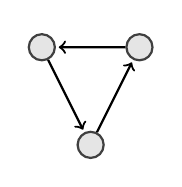
\begin{tikzpicture}[shorten >=1pt,->,scale=0.62]  
        \tikzstyle{sentence}=[circle,thick,draw=black!75,fill=black!10,minimum size=2mm]
        \tikzstyle{edge}=[draw, thick]
       \begin{scope}
         \node [sentence] (s1) at (0,2) {\tiny{}};
         \node [sentence] (s2) at (2,2) {\tiny{}};
         \node [sentence] (s3) at (1,0) {\tiny{}}; 
         
         \path[edge] (s2) edge [above] node[font=\tiny] {} (s1);
         \path[edge] (s1) edge [above] node[font=\tiny] {} (s3);
         \path[edge] (s3) edge [above] node[font=\tiny] {} (s2);
         
        \end{scope}        
      \end{tikzpicture}  
\\

&
 %%%%%%%%%%%%%%%%%%%%%%%%%%%%%% subgraph 9 %%%%%%%%%%%%%%%%%%%%%%%%%%%%%%
 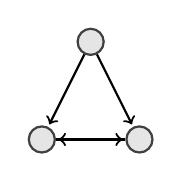
\begin{tikzpicture}[shorten >=1pt,->,scale=0.62]  
        \tikzstyle{sentence}=[circle,thick,draw=black!75,fill=black!10,minimum size=2mm]
        \tikzstyle{edge}=[draw, thick]
       \begin{scope}
         \node [sentence] (s1) at (1,2) {\tiny{}};
         \node [sentence] (s2) at (0,0) {\tiny{}};
         \node [sentence] (s3) at (2,0) {\tiny{}}; 
         
         \path[edge] (s1) edge [above] node[font=\tiny] {} (s2);
         \path[edge] (s1) edge [above] node[font=\tiny] {} (s3);
         \path[edge] (s3) edge [above] node[font=\tiny] {} (s2);
         \path[edge] (s2) edge [above] node[font=\tiny] {} (s3);
         
        \end{scope}        
      \end{tikzpicture}             
&
%%%%%%%%%%%%%%%%%%%%%%%%%%%%%% subgraph 10 %%%%%%%%%%%%%%%%%%%%%%%%%%%%%%
 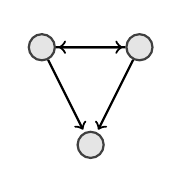
\begin{tikzpicture}[shorten >=1pt,->,scale=0.62]  
        \tikzstyle{sentence}=[circle,thick,draw=black!75,fill=black!10,minimum size=2mm]
        \tikzstyle{edge}=[draw, thick]
       \begin{scope}
         \node [sentence] (s1) at (0,2) {\tiny{}};
         \node [sentence] (s2) at (2,2) {\tiny{}};
         \node [sentence] (s3) at (1,0) {\tiny{}}; 
         
         \path[edge] (s1) edge [above] node[font=\tiny] {} (s2);
         \path[edge] (s2) edge [above] node[font=\tiny] {} (s1);
         \path[edge] (s1) edge [above] node[font=\tiny] {} (s3);
         \path[edge] (s2) edge [above] node[font=\tiny] {} (s3);
         
        \end{scope}        
      \end{tikzpicture}  

 &
 %%%%%%%%%%%%%%%%%%%%%%%%%%%%%% subgraph 11 %%%%%%%%%%%%%%%%%%%%%%%%%%%%%%
 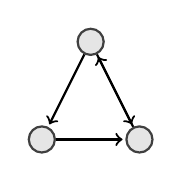
\begin{tikzpicture}[shorten >=1pt,->,scale=0.62]  
        \tikzstyle{sentence}=[circle,thick,draw=black!75,fill=black!10,minimum size=2mm]
        \tikzstyle{edge}=[draw, thick]
       \begin{scope}
         \node [sentence] (s1) at (1,2) {\tiny{}};
         \node [sentence] (s2) at (0,0) {\tiny{}};
         \node [sentence] (s3) at (2,0) {\tiny{}}; 
         
         \path[edge] (s1) edge [above] node[font=\tiny] {} (s2);
         \path[edge] (s1) edge [above] node[font=\tiny] {} (s3);
         \path[edge] (s3) edge [above] node[font=\tiny] {} (s1);
         \path[edge] (s2) edge [above] node[font=\tiny] {} (s3);
         
        \end{scope}        
      \end{tikzpicture}             

&
%%%%%%%%%%%%%%%%%%%%%%%%%%%%%% subgraph 12 %%%%%%%%%%%%%%%%%%%%%%%%%%%%%%
 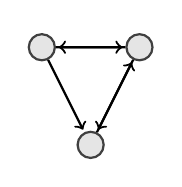
\begin{tikzpicture}[shorten >=1pt,->,scale=0.62]  
        \tikzstyle{sentence}=[circle,thick,draw=black!75,fill=black!10,minimum size=2mm]
        \tikzstyle{edge}=[draw, thick]
       \begin{scope}
         \node [sentence] (s1) at (0,2) {\tiny{}};
         \node [sentence] (s2) at (2,2) {\tiny{}};
         \node [sentence] (s3) at (1,0) {\tiny{}}; 
         
         \path[edge] (s1) edge [above] node[font=\tiny] {} (s2);
         \path[edge] (s2) edge [above] node[font=\tiny] {} (s1);
         \path[edge] (s1) edge [above] node[font=\tiny] {} (s3);
         \path[edge] (s2) edge [above] node[font=\tiny] {} (s3);
         \path[edge] (s3) edge [above] node[font=\tiny] {} (s2);
         
        \end{scope}        
      \end{tikzpicture}  
&
%%%%%%%%%%%%%%%%%%%%%%%%%%%%%% subgraph 13 %%%%%%%%%%%%%%%%%%%%%%%%%%%%%%
 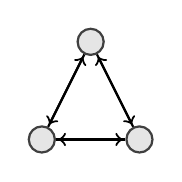
\begin{tikzpicture}[shorten >=1pt,->,scale=0.62]  
        \tikzstyle{sentence}=[circle,thick,draw=black!75,fill=black!10,minimum size=2mm]
        \tikzstyle{edge}=[draw, thick]
       \begin{scope}
         \node [sentence] (s1) at (1,2) {\tiny{}};
         \node [sentence] (s2) at (0,0) {\tiny{}};
         \node [sentence] (s3) at (2,0) {\tiny{}}; 
         
         \path[edge] (s1) edge [above] node[font=\tiny] {} (s2);
         \path[edge] (s2) edge [above] node[font=\tiny] {} (s1);

         \path[edge] (s2) edge [above] node[font=\tiny] {} (s3);
         \path[edge] (s3) edge [above] node[font=\tiny] {} (s2);
         
         \path[edge] (s1) edge [above] node[font=\tiny] {} (s3);
         \path[edge] (s3) edge [above] node[font=\tiny] {} (s1);
         
        \end{scope}        
      \end{tikzpicture} 
      &
      
\end{tabular}
}
\caption{All possible directed 3\-- node subgraphs.}
\label{f:all_3node_subgraphs}
\end{figure}

\textbf{Frequent large subgraphs.} Since we observe a strong correlation between basic subgraphs and human readability ratings
(Table \ref{t:comp_3node_pearson}), we mine frequent large subgraphs of projection graphs. 
Our intuition is that larger subgraphs are more informative coherence patterns. 
Hence, we extend the coherence features from all feasible 3-node subgraphs to frequent k-node subgraphs. 
We first use an efficient subgraph mining algorithm to extract all subgraphs with size $k$ and then compute the count of each subgraph as an induced subgraph in each graph $G\in\zeta$. 
We retain a subgraph $sg$, if it is frequent (i.e.\ $support(sg)>\lambda$). 
The result of these steps is a two-dimensional matrix whose rows represent graphs in $\zeta$ and columns represent frequent subgraphs with size $k$. 
The cell $\langle G_i,sg_j\rangle$ shows the count of $sg_j$ in graph $G_i$. Given this matrix, we compute the graph signature of each $G\in\zeta$ and take
each element of the graph signature as a coherence feature.




\section{Coherence Modeling}
\label{sec:automatic_extraction}



\section{Experiments}
\label{sec:experiments}

    \subsection{Readability Assessment}
    \label{subsec:readability_assessment}


        Readability depends on many factors which enable readers to process a text. 
        These factors can be used by readability assessment methods to quantify the difficulty of text understanding. 
        Possible applications of readability assessment are automatic text summarization and simplification systems. Measuring readability can also be used in
        question answering and knowledge extraction systems to prune texts with low readability \cite{kate10}.
        
        Many different text features have been used to assess readability. 
        They include shallow features \cite{flesch48,kincaid75}, language modeling features \cite{siluo01,collins-thompson04}, syntactic features \cite{schwarm05} and text flow or coherence \cite{barzilay08,pitler08}. 
        In a coherent text each sentence has some connections with other sentences. 
        Although these local connections make the text more readable, the corresponding coherence features used
        in \newcite{pitler08} (Section \ref{sec:readability_assessment}) are not strongly correlated with human judgments.


            \subsubsection{Data}
            %
            We use the dataset created by \newcite{pitler08} which consists of randomly selected articles from the Wall Street Journal corpus. 
            The articles were rated by three humans on a scale from $1$ to $5$ for readability based on quality measures that are designed to estimate the coherence of articles. The final readability score of each article is the average of these three ratings.
            
            We exclude three files from this dataset: \texttt{wsj\--0382} does not exist in the Penn Treebank \cite{marcus94}\footnote{\newcite{pitler08} also remove one file from their experiments. 
            We assume that it is  \texttt{wsj\--0382}.}. \texttt{wsj\--2090} does not exist in the Penn Discource Treebank \cite{prasad08a}. \texttt{wsj\--1398} is a poem.




% These patterns are encoded as subgraphs in graphs. 
% An advantage is that coherence can be measured beyond simple sentence or node connectivity.  

\subsubsection{Settings}
%



\textbf{Frequent subgraphs.} Since subgraph mining is an NP-complete problem, different algorithms have been introduced to
improve the performance of subgraph mining. 
We use the gSpan\footnote{We use the Java package: \url{http://www.cs.ucsb.edu/~xyan/software/gSpan.htm}} algorithm \cite{yanxifeng02} to mine subgraphs of a graph dataset which contains $P_u^{ER}$ projections. 
An advantage of using efficient subgraph mining algorithms is that we can exhaustively search very large subgraph spaces. 
A graph with $\Vert E \Vert$ edges, however, potentially has $\mathcal{O}(2^{\Vert E \Vert})$ subgraphs. 
Having sparse graphs and using efficient subgraph mining algorithm lets us to search trough this space. 
We mine subgraphs with $k=4$. (Figure \ref{4node_subgraphs}).




%\begin{figure}[!t]
%\centering
\small
\resizebox{1.0\columnwidth}{!}{
%\begin{tabular}{@{\hskip -1ex}c@{\hskip 1ex}c@{\hskip 1ex}c@{\hskip 1ex}c@{}}
\begin{tabular}{cccc}
\scriptsize{$sg_1$} & \scriptsize{$sg_2$} & \scriptsize{$sg_3$} & \scriptsize{$sg_4$}
\\
 %%%%%%%%%%%%%%%%%%%%%%%%%%%%%% sg 1 = 73 %%%%%%%%%%%%%%%%%%%%%%%%%%%%%%
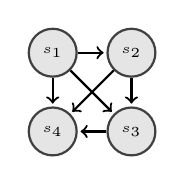
\begin{tikzpicture}[shorten >=1pt,->,scale=0.5]  
        \tikzstyle{sentence}=[circle,thick,draw=black!75,fill=black!10,minimum size=1mm]
        \tikzstyle{edge}=[draw, thick]
       \begin{scope}
         \node [sentence] (s1) at (0,2) {\tiny{$s_1$}};
         \node [sentence] (s2) at (2,2) {\tiny{$s_2$}};
         \node [sentence] (s3) at (2,0) {\tiny{$s_3$}};
         \node [sentence] (s4) at (0,0) {\tiny{$s_4$}};  
         \path[edge] (s1) edge [above] node[font=\tiny] {} (s2);
         \path[edge] (s1) edge [above] node[font=\tiny] {} (s3);
         \path[edge] (s1) edge [above] node[font=\tiny] {} (s4);
         \path[edge] (s2) edge [above] node[font=\tiny] {} (s4);
         \path[edge] (s2) edge [above] node[font=\tiny] {} (s3);
         \path[edge] (s3) edge [above] node[font=\tiny] {} (s4);
        \end{scope}        
      \end{tikzpicture}
&
%%%%%%%%%%%%%%%%%%%%%%%%%%%%%% sg 2 = 74 %%%%%%%%%%%%%%%%%%%%%%%%%%%%%%
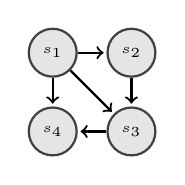
\begin{tikzpicture}[shorten >=1pt,->,scale=0.5]  
        \tikzstyle{sentence}=[circle,thick,draw=black!75,fill=black!10,minimum size=2mm]
        \tikzstyle{edge}=[draw, thick]
       \begin{scope}
         \node [sentence] (s1) at (0,2) {\tiny{$s_1$}};
         \node [sentence] (s2) at (2,2) {\tiny{$s_2$}};
         \node [sentence] (s3) at (2,0) {\tiny{$s_3$}};
         \node [sentence] (s4) at (0,0) {\tiny{$s_4$}};  
         \path[edge] (s1) edge [above] node[font=\tiny] {} (s2);
         \path[edge] (s1) edge [above] node[font=\tiny] {} (s3);
         \path[edge] (s1) edge [above] node[font=\tiny] {} (s4);
         \path[edge] (s2) edge [above] node[font=\tiny] {} (s3);
         \path[edge] (s3) edge [above] node[font=\tiny] {} (s4);
        \end{scope}        
      \end{tikzpicture}
&
%%%%%%%%%%%%%%%%%%%%%%%%%%%%%% sg 3 = 83 %%%%%%%%%%%%%%%%%%%%%%%%%%%%%%
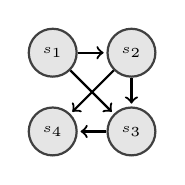
\begin{tikzpicture}[shorten >=1pt,->,scale=0.5]  
        \tikzstyle{sentence}=[circle,thick,draw=black!75,fill=black!10,minimum size=2mm]
        \tikzstyle{edge}=[draw, thick]
       \begin{scope}
         \node [sentence] (s1) at (0,2) {\tiny{$s_1$}};
         \node [sentence] (s2) at (2,2) {\tiny{$s_2$}};
         \node [sentence] (s3) at (2,0) {\tiny{$s_3$}};
         \node [sentence] (s4) at (0,0) {\tiny{$s_4$}};  
         \path[edge] (s1) edge [above] node[font=\tiny] {} (s2);
         \path[edge] (s1) edge [above] node[font=\tiny] {} (s3);
         \path[edge] (s2) edge [above] node[font=\tiny] {} (s3);
         \path[edge] (s2) edge [above] node[font=\tiny] {} (s4);
         \path[edge] (s3) edge [above] node[font=\tiny] {} (s4);
        \end{scope}        
      \end{tikzpicture}
&
%%%%%%%%%%%%%%%%%%%%%%%%%%%%%% sg 4 =84 %%%%%%%%%%%%%%%%%%%%%%%%%%%%%%
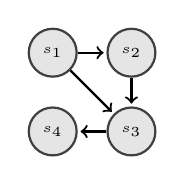
\begin{tikzpicture}[shorten >=1pt,->,scale=0.5]  
        \tikzstyle{sentence}=[circle,thick,draw=black!75,fill=black!10,minimum size=2mm]
        \tikzstyle{edge}=[draw, thick]
       \begin{scope}
         \node [sentence] (s1) at (0,2) {\tiny{$s_1$}};
         \node [sentence] (s2) at (2,2) {\tiny{$s_2$}};
         \node [sentence] (s3) at (2,0) {\tiny{$s_3$}};
         \node [sentence] (s4) at (0,0) {\tiny{$s_4$}};  
         \path[edge] (s1) edge [above] node[font=\tiny] {} (s2);
         \path[edge] (s1) edge [above] node[font=\tiny] {} (s3);
         \path[edge] (s2) edge [above] node[font=\tiny] {} (s3);
         \path[edge] (s3) edge [above] node[font=\tiny] {} (s4);
        \end{scope}        
      \end{tikzpicture}
\\
\scriptsize{$sg_5$} & \scriptsize{$sg_6$} & \scriptsize{$sg_7$} & \scriptsize{$sg_8$}
\\
%%%%%%%%%%%%%%%%%%%%%%%%%%%%%% sg 5 = 106 %%%%%%%%%%%%%%%%%%%%%%%%%%%%%%
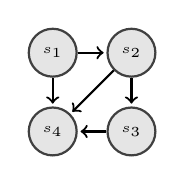
\begin{tikzpicture}[shorten >=1pt,->,scale=0.5]  
        \tikzstyle{sentence}=[circle,thick,draw=black!75,fill=black!10,minimum size=2mm]
        \tikzstyle{edge}=[draw, thick]
       \begin{scope}
         \node [sentence] (s1) at (0,2) {\tiny{$s_1$}};
         \node [sentence] (s2) at (2,2) {\tiny{$s_2$}};
         \node [sentence] (s3) at (2,0) {\tiny{$s_3$}};
         \node [sentence] (s4) at (0,0) {\tiny{$s_4$}};  
         \path[edge] (s1) edge [above] node[font=\tiny] {} (s2);
         \path[edge] (s1) edge [above] node[font=\tiny] {} (s4);
         \path[edge] (s2) edge [above] node[font=\tiny] {} (s3);
         \path[edge] (s2) edge [above] node[font=\tiny] {} (s4);
         \path[edge] (s3) edge [above] node[font=\tiny] {} (s4);
        \end{scope}        
      \end{tikzpicture}
&
%%%%%%%%%%%%%%%%%%%%%%%%%%%%%% sg 6 = 117 %%%%%%%%%%%%%%%%%%%%%%%%%%%%%%
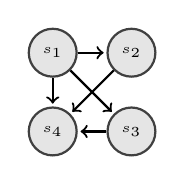
\begin{tikzpicture}[shorten >=1pt,->,scale=0.5]  
        \tikzstyle{sentence}=[circle,thick,draw=black!75,fill=black!10,minimum size=2mm]
        \tikzstyle{edge}=[draw, thick]
       \begin{scope}
         \node [sentence] (s1) at (0,2) {\tiny{$s_1$}};
         \node [sentence] (s2) at (2,2) {\tiny{$s_2$}};
         \node [sentence] (s3) at (2,0) {\tiny{$s_3$}};
         \node [sentence] (s4) at (0,0) {\tiny{$s_4$}};  
         \path[edge] (s1) edge [above] node[font=\tiny] {} (s2);
         \path[edge] (s1) edge [above] node[font=\tiny] {} (s3);
         \path[edge] (s1) edge [above] node[font=\tiny] {} (s4);
         \path[edge] (s2) edge [above] node[font=\tiny] {} (s4);
         \path[edge] (s3) edge [above] node[font=\tiny] {} (s4);

        \end{scope}        
      \end{tikzpicture}
&
%%%%%%%%%%%%%%%%%%%%%%%%%%%%%% sg 7 =126 %%%%%%%%%%%%%%%%%%%%%%%%%%%%%%
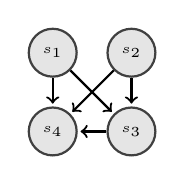
\begin{tikzpicture}[shorten >=1pt,->,scale=0.5]  
        \tikzstyle{sentence}=[circle,thick,draw=black!75,fill=black!10,minimum size=2mm]
        \tikzstyle{edge}=[draw, thick]
       \begin{scope}
         \node [sentence] (s1) at (0,2) {\tiny{$s_1$}};
         \node [sentence] (s2) at (2,2) {\tiny{$s_2$}};
         \node [sentence] (s3) at (2,0) {\tiny{$s_3$}};
         \node [sentence] (s4) at (0,0) {\tiny{$s_4$}};  
         \path[edge] (s1) edge [above] node[font=\tiny] {} (s3);
         \path[edge] (s1) edge [above] node[font=\tiny] {} (s4);
         \path[edge] (s2) edge [above] node[font=\tiny] {} (s3);
         \path[edge] (s2) edge [above] node[font=\tiny] {} (s4);
         \path[edge] (s3) edge [above] node[font=\tiny] {} (s4);
        \end{scope}        
      \end{tikzpicture}
&
%%%%%%%%%%%%%%%%%%%%%%%%%%%%%% sg 8 = 127 %%%%%%%%%%%%%%%%%%%%%%%%%%%%%%
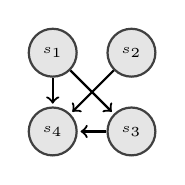
\begin{tikzpicture}[shorten >=1pt,->,scale=0.5]  
        \tikzstyle{sentence}=[circle,thick,draw=black!75,fill=black!10,minimum size=2mm]
        \tikzstyle{edge}=[draw, thick]
       \begin{scope}
         \node [sentence] (s1) at (0,2) {\tiny{$s_1$}};
         \node [sentence] (s2) at (2,2) {\tiny{$s_2$}};
         \node [sentence] (s3) at (2,0) {\tiny{$s_3$}};
         \node [sentence] (s4) at (0,0) {\tiny{$s_4$}};  
         \path[edge] (s1) edge [above] node[font=\tiny] {} (s3);
         \path[edge] (s1) edge [above] node[font=\tiny] {} (s4);
         \path[edge] (s2) edge [above] node[font=\tiny] {} (s4);
         \path[edge] (s3) edge [above] node[font=\tiny] {} (s4);
        \end{scope}        
      \end{tikzpicture}
\\
\scriptsize{$sg_9$} & \scriptsize{$sg_{10}$} & \scriptsize{$sg_{11}$} & \scriptsize{$sg_{12}$}
\\


%%%%%%%%%%%%%%%%%%%%%%%%%%%%%% sg 9 =145 %%%%%%%%%%%%%%%%%%%%%%%%%%%%%%
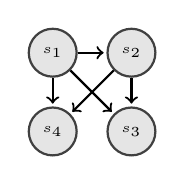
\begin{tikzpicture}[shorten >=1pt,->,scale=0.5]  
        \tikzstyle{sentence}=[circle,thick,draw=black!75,fill=black!10,minimum size=2mm]
        \tikzstyle{edge}=[draw, thick]
       \begin{scope}
         \node [sentence] (s1) at (0,2) {\tiny{$s_1$}};
         \node [sentence] (s2) at (2,2) {\tiny{$s_2$}};
         \node [sentence] (s3) at (2,0) {\tiny{$s_3$}};
         \node [sentence] (s4) at (0,0) {\tiny{$s_4$}};  
         \path[edge] (s1) edge [above] node[font=\tiny] {} (s2);
         \path[edge] (s1) edge [above] node[font=\tiny] {} (s3);
         \path[edge] (s1) edge [above] node[font=\tiny] {} (s4);
         \path[edge] (s2) edge [above] node[font=\tiny] {} (s3);
         \path[edge] (s2) edge [above] node[font=\tiny] {} (s4);
        \end{scope}        
      \end{tikzpicture}
&
%%%%%%%%%%%%%%%%%%%%%%%%%%%%%% sg 10  = 146 %%%%%%%%%%%%%%%%%%%%%%%%%%%%%%
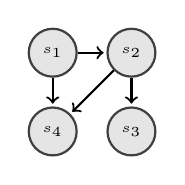
\begin{tikzpicture}[shorten >=1pt,->,scale=0.5]  
        \tikzstyle{sentence}=[circle,thick,draw=black!75,fill=black!10,minimum size=2mm]
        \tikzstyle{edge}=[draw, thick]
       \begin{scope}
         \node [sentence] (s1) at (0,2) {\tiny{$s_1$}};
         \node [sentence] (s2) at (2,2) {\tiny{$s_2$}};
         \node [sentence] (s3) at (2,0) {\tiny{$s_3$}};
         \node [sentence] (s4) at (0,0) {\tiny{$s_4$}};  
         \path[edge] (s1) edge [above] node[font=\tiny] {} (s2);
         \path[edge] (s1) edge [above] node[font=\tiny] {} (s4);
         \path[edge] (s2) edge [above] node[font=\tiny] {} (s3);
         \path[edge] (s2) edge [above] node[font=\tiny] {} (s4);
        \end{scope}        
      \end{tikzpicture}
&
%%%%%%%%%%%%%%%%%%%%%%%%%%%%%% sg 11  = 156 %%%%%%%%%%%%%%%%%%%%%%%%%%%%%%
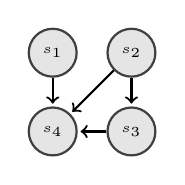
\begin{tikzpicture}[shorten >=1pt,->,scale=0.5]  
        \tikzstyle{sentence}=[circle,thick,draw=black!75,fill=black!10,minimum size=2mm]
        \tikzstyle{edge}=[draw, thick]
       \begin{scope}
         \node [sentence] (s1) at (0,2) {\tiny{$s_1$}};
         \node [sentence] (s2) at (2,2) {\tiny{$s_2$}};
         \node [sentence] (s3) at (2,0) {\tiny{$s_3$}};
         \node [sentence] (s4) at (0,0) {\tiny{$s_4$}};  
         \path[edge] (s1) edge [above] node[font=\tiny] {} (s4);
         \path[edge] (s2) edge [above] node[font=\tiny] {} (s3);
         \path[edge] (s2) edge [above] node[font=\tiny] {} (s4);
         \path[edge] (s3) edge [above] node[font=\tiny] {} (s4);
        \end{scope}        
      \end{tikzpicture}
&
%%%%%%%%%%%%%%%%%%%%%%%%%%%%%% sg 12 = 165 %%%%%%%%%%%%%%%%%%%%%%%%%%%%%%
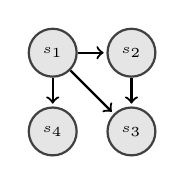
\begin{tikzpicture}[shorten >=1pt,->,scale=0.5]  
        \tikzstyle{sentence}=[circle,thick,draw=black!75,fill=black!10,minimum size=2mm]
        \tikzstyle{edge}=[draw, thick]
       \begin{scope}
         \node [sentence] (s1) at (0,2) {\tiny{$s_1$}};
         \node [sentence] (s2) at (2,2) {\tiny{$s_2$}};
         \node [sentence] (s3) at (2,0) {\tiny{$s_3$}};
         \node [sentence] (s4) at (0,0) {\tiny{$s_4$}};  
         \path[edge] (s1) edge [above] node[font=\tiny] {} (s2);
         \path[edge] (s1) edge [above] node[font=\tiny] {} (s3);
         \path[edge] (s1) edge [above] node[font=\tiny] {} (s4);
         \path[edge] (s2) edge [above] node[font=\tiny] {} (s3);
        \end{scope}        
      \end{tikzpicture}
\\
\scriptsize{$sg_{13}$} & \scriptsize{$sg_{14}$} & \scriptsize{$sg_{15}$} & \scriptsize{$sg_{16}$}
\\

%%%%%%%%%%%%%%%%%%%%%%%%%%%%%% sg 13 = 172 %%%%%%%%%%%%%%%%%%%%%%%%%%%%%%
\begin{tikzpicture}[shorten >=1pt,->,scale=0.5]  
        \tikzstyle{sentence}=[circle,thick,draw=black!75,fill=black!10,minimum size=2mm]
        \tikzstyle{edge}=[draw, thick]
       \begin{scope}
         \node [sentence] (s1) at (0,2) {\tiny{$s_1$}};
         \node [sentence] (s2) at (2,2) {\tiny{$s_2$}};
         \node [sentence] (s3) at (2,0) {\tiny{$s_3$}};
         \node [sentence] (s4) at (0,0) {\tiny{$s_4$}};  
         \path[edge] (s1) edge [above] node[font=\tiny] {} (s2);
         \path[edge] (s2) edge [above] node[font=\tiny] {} (s3);
         \path[edge] (s2) edge [above] node[font=\tiny] {} (s4);
         \path[edge] (s3) edge [above] node[font=\tiny] {} (s4);
        \end{scope}        
      \end{tikzpicture}
&
%%%%%%%%%%%%%%%%%%%%%%%%%%%%%% sg 14 =192 %%%%%%%%%%%%%%%%%%%%%%%%%%%%%%
\begin{tikzpicture}[shorten >=1pt,->,scale=0.5]  
        \tikzstyle{sentence}=[circle,thick,draw=black!75,fill=black!10,minimum size=2mm]
        \tikzstyle{edge}=[draw, thick]
       \begin{scope}
         \node [sentence] (s1) at (0,2) {\tiny{$s_1$}};
         \node [sentence] (s2) at (2,2) {\tiny{$s_2$}};
         \node [sentence] (s3) at (2,0) {\tiny{$s_3$}};
         \node [sentence] (s4) at (0,0) {\tiny{$s_4$}};  
         \path[edge] (s1) edge [above] node[font=\tiny] {} (s2);
         \path[edge] (s1) edge [above] node[font=\tiny] {} (s4);
         \path[edge] (s2) edge [above] node[font=\tiny] {} (s3);
         \path[edge] (s3) edge [above] node[font=\tiny] {} (s4);
        \end{scope}        
      \end{tikzpicture}
&
%%%%%%%%%%%%%%%%%%%%%%%%%%%%%% sg 15 =193 %%%%%%%%%%%%%%%%%%%%%%%%%%%%%%
\begin{tikzpicture}[shorten >=1pt,->,scale=0.5]  
        \tikzstyle{sentence}=[circle,thick,draw=black!75,fill=black!10,minimum size=2mm]
        \tikzstyle{edge}=[draw, thick]
       \begin{scope}
         \node [sentence] (s1) at (0,2) {\tiny{$s_1$}};
         \node [sentence] (s2) at (2,2) {\tiny{$s_2$}};
         \node [sentence] (s3) at (2,0) {\tiny{$s_3$}};
         \node [sentence] (s4) at (0,0) {\tiny{$s_4$}};  
         \path[edge] (s1) edge [above] node[font=\tiny] {} (s2);
         \path[edge] (s2) edge [above] node[font=\tiny] {} (s3);
         \path[edge] (s3) edge [above] node[font=\tiny] {} (s4);
        \end{scope}        
      \end{tikzpicture}
&
%%%%%%%%%%%%%%%%%%%%%%%%%%%%%% sg 16 = 216 %%%%%%%%%%%%%%%%%%%%%%%%%%%%%%
\begin{tikzpicture}[shorten >=1pt,->,scale=0.5]  
        \tikzstyle{sentence}=[circle,thick,draw=black!75,fill=black!10,minimum size=2mm]
        \tikzstyle{edge}=[draw, thick]
       \begin{scope}
         \node [sentence] (s1) at (0,2) {\tiny{$s_1$}};
         \node [sentence] (s2) at (2,2) {\tiny{$s_2$}};
         \node [sentence] (s3) at (2,0) {\tiny{$s_3$}};
         \node [sentence] (s4) at (0,0) {\tiny{$s_4$}};  
         \path[edge] (s1) edge [above] node[font=\tiny] {} (s2);
         \path[edge] (s1) edge [above] node[font=\tiny] {} (s3);
         \path[edge] (s2) edge [above] node[font=\tiny] {} (s4);
         \path[edge] (s3) edge [above] node[font=\tiny] {} (s4);
        \end{scope}        
      \end{tikzpicture}
\\
\scriptsize{$sg_{17}$} & \scriptsize{$sg_{18}$} & \scriptsize{$sg_{19}$} & \scriptsize{$sg_{20}$}
\\

%%%%%%%%%%%%%%%%%%%%%%%%%%%%%% sg 17 = 217 %%%%%%%%%%%%%%%%%%%%%%%%%%%%%%
\begin{tikzpicture}[shorten >=1pt,->,scale=0.5]  
        \tikzstyle{sentence}=[circle,thick,draw=black!75,fill=black!10,minimum size=2mm]
        \tikzstyle{edge}=[draw, thick]
       \begin{scope}
         \node [sentence] (s1) at (0,2) {\tiny{$s_1$}};
         \node [sentence] (s2) at (2,2) {\tiny{$s_2$}};
         \node [sentence] (s3) at (2,0) {\tiny{$s_3$}};
         \node [sentence] (s4) at (0,0) {\tiny{$s_4$}};  
         \path[edge] (s1) edge [above] node[font=\tiny] {} (s4);
         \path[edge] (s2) edge [above] node[font=\tiny] {} (s3);
         \path[edge] (s3) edge [above] node[font=\tiny] {} (s4);
        \end{scope}        
      \end{tikzpicture}

&
%%%%%%%%%%%%%%%%%%%%%%%%%%%%%% sg 18 = 227 %%%%%%%%%%%%%%%%%%%%%%%%%%%%%%
\begin{tikzpicture}[shorten >=1pt,->,scale=0.5]  
        \tikzstyle{sentence}=[circle,thick,draw=black!75,fill=black!10,minimum size=2mm]
        \tikzstyle{edge}=[draw, thick]
       \begin{scope}
         \node [sentence] (s1) at (0,2) {\tiny{$s_1$}};
         \node [sentence] (s2) at (2,2) {\tiny{$s_2$}};
         \node [sentence] (s3) at (2,0) {\tiny{$s_3$}};
         \node [sentence] (s4) at (0,0) {\tiny{$s_4$}};  
         \path[edge] (s1) edge [above] node[font=\tiny] {} (s2);
         \path[edge] (s2) edge [above] node[font=\tiny] {} (s3);
         \path[edge] (s2) edge [above] node[font=\tiny] {} (s4);
        \end{scope}        
      \end{tikzpicture}

&
%%%%%%%%%%%%%%%%%%%%%%%%%%%%%% sg 19 =237 %%%%%%%%%%%%%%%%%%%%%%%%%%%%%%
\begin{tikzpicture}[shorten >=1pt,->,scale=0.5]  
        \tikzstyle{sentence}=[circle,thick,draw=black!75,fill=black!10,minimum size=2mm]
        \tikzstyle{edge}=[draw, thick]
       \begin{scope}
         \node [sentence] (s1) at (0,2) {\tiny{$s_1$}};
         \node [sentence] (s2) at (2,2) {\tiny{$s_2$}};
         \node [sentence] (s3) at (2,0) {\tiny{$s_3$}};
         \node [sentence] (s4) at (0,0) {\tiny{$s_4$}};  
         \path[edge] (s1) edge [above] node[font=\tiny] {} (s3);
         \path[edge] (s2) edge [above] node[font=\tiny] {} (s3);
         \path[edge] (s3) edge [above] node[font=\tiny] {} (s4);
        \end{scope}        
      \end{tikzpicture}
&
%%%%%%%%%%%%%%%%%%%%%%%%%%%%%% sg 20 =246 %%%%%%%%%%%%%%%%%%%%%%%%%%%%%%
\begin{tikzpicture}[shorten >=1pt,->,scale=0.5]  
        \tikzstyle{sentence}=[circle,thick,draw=black!75,fill=black!10,minimum size=2mm]
        \tikzstyle{edge}=[draw, thick]
       \begin{scope}
         \node [sentence] (s1) at (0,2) {\tiny{$s_1$}};
         \node [sentence] (s2) at (2,2) {\tiny{$s_2$}};
         \node [sentence] (s3) at (2,0) {\tiny{$s_3$}};
         \node [sentence] (s4) at (0,0) {\tiny{$s_4$}};  
         \path[edge] (s1) edge [above] node[font=\tiny] {} (s3);
         \path[edge] (s1) edge [above] node[font=\tiny] {} (s2);
         \path[edge] (s3) edge [above] node[font=\tiny] {} (s4);
        \end{scope}        
      \end{tikzpicture}
\\
\scriptsize{$sg_{21}$} & \scriptsize{$sg_{22}$} & \scriptsize{$sg_{23}$} & \scriptsize{$sg_{24}$}
\\

%%%%%%%%%%%%%%%%%%%%%%%%%%%%%% sg 21 =277 %%%%%%%%%%%%%%%%%%%%%%%%%%%%%%
\begin{tikzpicture}[shorten >=1pt,->,scale=0.5]  
        \tikzstyle{sentence}=[circle,thick,draw=black!75,fill=black!10,minimum size=2mm]
        \tikzstyle{edge}=[draw, thick]
       \begin{scope}
         \node [sentence] (s1) at (0,2) {\tiny{$s_1$}};
         \node [sentence] (s2) at (2,2) {\tiny{$s_2$}};
         \node [sentence] (s3) at (2,0) {\tiny{$s_3$}};
         \node [sentence] (s4) at (0,0) {\tiny{$s_4$}};  
         \path[edge] (s1) edge [above] node[font=\tiny] {} (s3);
         \path[edge] (s1) edge [above] node[font=\tiny] {} (s4);
         \path[edge] (s2) edge [above] node[font=\tiny] {} (s3);
         \path[edge] (s2) edge [above] node[font=\tiny] {} (s4);
        \end{scope}        
      \end{tikzpicture}
&
%%%%%%%%%%%%%%%%%%%%%%%%%%%%%% sg 22 =278 %%%%%%%%%%%%%%%%%%%%%%%%%%%%%%
\begin{tikzpicture}[shorten >=1pt,->,scale=0.5]  
        \tikzstyle{sentence}=[circle,thick,draw=black!75,fill=black!10,minimum size=2mm]
        \tikzstyle{edge}=[draw, thick]
       \begin{scope}
         \node [sentence] (s1) at (0,2) {\tiny{$s_1$}};
         \node [sentence] (s2) at (2,2) {\tiny{$s_2$}};
         \node [sentence] (s3) at (2,0) {\tiny{$s_3$}};
         \node [sentence] (s4) at (0,0) {\tiny{$s_4$}};  
         \path[edge] (s1) edge [above] node[font=\tiny] {} (s3);
         \path[edge] (s1) edge [above] node[font=\tiny] {} (s4);
         \path[edge] (s2) edge [above] node[font=\tiny] {} (s4);
        \end{scope}        
      \end{tikzpicture}

&
%%%%%%%%%%%%%%%%%%%%%%%%%%%%%% sg 23 = 289  %%%%%%%%%%%%%%%%%%%%%%%%%%%%%%
\begin{tikzpicture}[shorten >=1pt,->,scale=0.5]  
        \tikzstyle{sentence}=[circle,thick,draw=black!75,fill=black!10,minimum size=2mm]
        \tikzstyle{edge}=[draw, thick]
       \begin{scope}
         \node [sentence] (s1) at (0,2) {\tiny{$s_1$}};
         \node [sentence] (s2) at (2,2) {\tiny{$s_2$}};
         \node [sentence] (s3) at (2,0) {\tiny{$s_3$}};
         \node [sentence] (s4) at (0,0) {\tiny{$s_4$}};  
         \path[edge] (s1) edge [above] node[font=\tiny] {} (s4);
         \path[edge] (s2) edge [above] node[font=\tiny] {} (s4);
         \path[edge] (s3) edge [above] node[font=\tiny] {} (s4);
        \end{scope}        
      \end{tikzpicture}

&
%%%%%%%%%%%%%%%%%%%%%%%%%%%%%% sg 24 = 304 %%%%%%%%%%%%%%%%%%%%%%%%%%%%%%
\begin{tikzpicture}[shorten >=1pt,->,scale=0.5]  
        \tikzstyle{sentence}=[circle,thick,draw=black!75,fill=black!10,minimum size=2mm]
        \tikzstyle{edge}=[draw, thick]
       \begin{scope}
         \node [sentence] (s1) at (0,2) {\tiny{$s_1$}};
         \node [sentence] (s2) at (2,2) {\tiny{$s_2$}};
         \node [sentence] (s3) at (2,0) {\tiny{$s_3$}};
         \node [sentence] (s4) at (0,0) {\tiny{$s_4$}};  
         \path[edge] (s1) edge [above] node[font=\tiny] {} (s2);
         \path[edge] (s1) edge [above] node[font=\tiny] {} (s3);
         \path[edge] (s1) edge [above] node[font=\tiny] {} (s4);
        \end{scope}        
      \end{tikzpicture}



\end{tabular}
}

%\caption{Frequent subgraphs with four nodes where $t<u<v<w$.}\label{4node_subgraphs}
%\end{figure}


%



\subsubsection{Results}\label{subsec:results}
%
\textbf{Readability assessment.}  
\noindent
\textbf{Readability assessment.} We use the Pearson correlation coefficient to find features correlated with readability scores. 
It takes feature values and readability scores of all articles and returns $-1\leq\rho\leq+1$. 
A high value of $|\rho|$ shows a strong correlation. 
We report statistical significance on the $0.05$-level. 
We report the correlation of our coherence models encoded in graph features and compare them with \newcite{guinaudeau13} entity graph as the state-of-the-art coherence model. 
\newcite{pitler08} show that the entity transition features extracted from the entity grid model \cite{barzilay08} on its own do not significantly predict human
readability ratings. 
So we do not describe their results here.

\begin{table}[!t]
\centering
\begin{small}
\begin{tabular}{lrc}
\hline
                        & $\rho$                & p\_value\\\hline
        \multicolumn{3}{l}{\textbf{Entity Graph}}\\
 $P_u^{ER}$             & $-0.013$ & 0.949 \\
 $P_w^{ER}$             & 0.151  & 0.452\\
 $P_{acc}^{ER}$ & 0.150         & 0.455\\
\hline
\multicolumn{3}{l}{\textbf{Discourse Relation Graph}}\\
 $P_u^{DR}$ &  0.150 & 0.455\\
 $P_w^{DR}$ &  0.155  & 0.440\\\hline
 \multicolumn{3}{l}{\textbf{Combination of Entity and Discourse Relation}}\\
 $P_u^{ER} \lor P_u^{DR}$  &  0.083 & 0.681\\
 $P_w^{ER} + P_u^{DR}$ & 0.185  & 0.356\\
 $P_w^{ER} + P_w^{DR}$ & 0.187  & 0.350\\\hline
\end{tabular}
\end{small}
\caption{The correlation of the average outdegree of different graphs with human readability ratings.}
  \label{t:OD_pearson}
\end{table}

The results for the outdegree feature is shown in Table \ref{t:OD_pearson}.
% The first section of the table shows the correlation of outdegree feature of three kinds of projections of the entity graph model. 
The average outdegree of $P_w^{ER}$ is highly correlated with human readability ratings. This confirms the readability results of
\newcite{guinaudeau13} on the Encyclopedia Britannica dataset. 
% The second section shows the correlation of the outdegree of unweighted $P_u^{DR}$ and weighted $P_w^{DR}$ discourse relation graphs. 
The outdegrees of discourse relation graphs are more strongly correlated with human readability ratings than the outdegree of the projections in the entity graph, suggesting that efficient graph-based encoding of discourse relations can measure readability well.
% The last section shows the result of the correlation of different combined graphs' outdegree. 
The outdegree of the combined graph $P_w^{ER}+P_w^{DR}$ is highly correlated, showing that the interaction of entity connections and discourse relations is important for text coherence.
% Moreover, getting higher correlation coefficient with combined graphs than the projections of entity graph and discourse relations graphs, saying that the entity graph model needs to enrich with semantical continuity relations and our combined models merge the entity graph with discourse relations as logical connections in a text. On the other hand
However, none of the outdegree measures in this table are significantly correlated with human readability ratings, confirming the intuition that outdegree only measures node connectivity in graphs and it is not enough to measure readability.

\begin{table}[!h]
\centering
\begin{small}
\begin{tabular}{lrc}
\hline
   & $\rho$ & p\_value\\\hline
\textbf{Number of Components}   &       $\mathbf{-0.391}$       &       \textbf{0.044}  \\\hline

\multicolumn{3}{l}{\textbf{Relative frequency of 3-node Subgraphs}} \\
 $sg_1$ &  0.310 & 0.116\\
 $sg_2$ & $-0.325$ & 0.098\\
$\mathbf{sg_3}$ & $\mathbf{-0.384}$ & \textbf{0.048}\\
 $sg_4$ &  0.108 & 0.592\\\hline
\end{tabular}
\end{small}
\caption{Number of components and subgraph $sg_3$ are significantly correlated to readability.}
  \label{t:comp_3node_pearson}
\end{table}

Table \ref{t:comp_3node_pearson} shows the correlation of two features of projections\footnote{Although, the proposed features can be applied on all kind of presented graphs, we evaluate them (except outdegree) only on projections of the entity graph model. 
We leave the application to the other graph representations for future work.}:
The number of components has a strong and significant negative correlation with human readability ratings\footnote{This supports
  \newcite{karamanis09} who report that NOCB transitions in the centering model can be used for the sentence ordering task.},
suggesting that simple properties of graphs measure text
coherence. 
The lower part of Table \ref{t:comp_3node_pearson} shows the correlation of the relative frequency of 3-node subgraphs (see Figure \ref{f:feasible_3node_subgraphs}).  
More readable articles have many $sg_1$ and few number of $sg_2$ patterns. 
Pattern $sg_3$ is significantly and negatively correlated with human readability judgments, confirming the intuition that many shifts in focus
of attention make texts difficult to read. 



\begin{table}[!t]
\centering
\begin{small}
\begin{tabular}{lcrc}
\hline
   & number of edges & $\rho$ & p\_value\\\hline
$sg_1$ & 6 & 0.103 & 0.609   \\
$sg_2$ & 5 & $-0.212$ & 0.288    \\
$sg_3$  & 5 &   $-0.176$ & 0.380      \\
$sg_4$  & 4 &$-0.257$ & 0.196    \\
$sg_5$ & 5 &$-0.140$ & 0. 486   \\
$sg_6$  & 5 &   0.200 &  0.317  \\
$\mathbf{sg_7}$ & \textbf{5} & $\mathbf{-0.402}$ & \textbf{0.038}  \\
$sg_8$  & 4 &$-0.317$ & 0.107 \\
$sg_9$ & 5 & 0.153 & 0.446   \\
$sg_{10}$ & 4 & $-0.238$ & 0.232    \\
$\mathbf{sg_{11}}$ & \textbf{4} & $\mathbf{-0.509}$     & \textbf{0.007}\\
$\mathbf{sg_{12}}$  & \textbf{4} &\textbf{0.449} & \textbf{0.019}    \\
$sg_{13}$  & 4 & $-0.045$ & 0.824    \\
$sg_{14}$ & 4 & $-0.033$ & 0.870\\
$sg_{15}$ & 3 &$-0.358$ & 0.067    \\
$sg_{16}$ &     4 &$-0.068$ & 0.736    \\
$sg_{17}$  & 3 & $-0.308$ & 0.118    \\
$\mathbf{sg_{18}}$ & \textbf{3} & $\mathbf{-0.546}$      & \textbf{0.003}   \\
$\mathbf{sg_{19}}$ & \textbf{3} & $\mathbf{-0.601}$ & \textbf{0.001}   \\
$sg_{20}$ & 3 & 0.094   & 0.641 \\
$sg_{21}$  & 4 & 0.068 & 0.736   \\
$sg_{22}$ &  3& $-0.374$ &  0.055  \\
$sg_{23}$ &     3&$-0.314$ & 0.111 \\
$sg_{24}$ &     3& 0.100 & 0.620  \\
\hline
\end{tabular}
\end{small}
\caption{The correlation between the relative frequency of 4-node subgraphs and readability ratings.}\label{t:correlation_4node_subgraph}
\end{table}


Table \ref{t:correlation_4node_subgraph} shows the correlation between the relative frequency of 4-node subgraphs and readability ratings. 
First, most subgraphs with less than four edges are negatively correlated with readability, except $sg_{20}$ and $sg_{24}$ which are weakly correlated with readability. Few connections between sentences make the text difficult to read.

Second, the highest positive and significant correlation of $sg_{12}$ and the most negatively correlated subgraph $sg_{11}$ show that different patterns of edges in subgraphs capture readability judgments. 
\newcite[p.29]{stoddard91} explains this by the \emph{ambiguity node}\ phenomenon: ``[...] in some cases, there may be more
than one logical, possible node for a given cohesive element in a text, in which case, a reader may see the resulting ambiguity but not be able to decide between the choices''. 
E.g., in $sg_{11}$ a reader may make a decision about the focus of attention in $s_w$, while in $sg_{12}$ the focus of attention of $s_w$ is the same as the
focus of attention of $s_t$. This phenomenon can also be observed in all positively correlated subgraphs. If readers have to return to one point in the text, they prefer to return to a sentence which is the core of the preceding sentences.
% Of course, it is difficult to interpret these patterns one by one, since in a graph they can occur  in different situations. But these analysis show that humans easily understand texts which contain many number of pattern $sg_{12}$.
However, we should refrain of interpreting too much into these patterns.

Finally, we conclude that in all strongly negative correlated subgraphs, a subgraph suffers either from edge shortage or the \textit{ambiguity node}\ phenomenon like $sg_7$.

Considering the correlation of 3-node subgraphs in Table \ref{t:comp_3node_pearson} and 4-node subgraphs in Table \ref{t:correlation_4node_subgraph}, two results are noticeable.
First, in large subgraphs there are more strongly correlated subgraphs than 3-node subgraphs, confirming our hypothesis that larger subgraphs convey coherence patterns with higher quality. Second, $sg_{12}$ in 4-node subgraphs is more strongly and positively correlated than $sg_4$ in 3-node subgraphs, because $sg_{12}$ captures more circumstances about $s_t$. 
The relative frequency of $sg_{12}$ is more informative than $sg_4$'s relative frequency.

\noindent
\textbf{Readability as ranking.} 

\textbf{Readability as ranking.} We rank texts pairwise with respect to their readability. 
We define a classification problem with a set of text pairs and a label, which indicates whether the first text in a pair is more readable. 
We use every two texts whose human readability scores differ by at least $0.5$. 
Each text is represented with its graph-based coherence features. 
We employ WEKA's linear support vector implementation (SMO)  to classify the pairs. 
Performance is evaluated using 10-fold cross-validation.

Results of the readability ranking problem are shown in Table \ref{t:classification_task}. 
Baseline features are entity transition features which are used as coherence features by \newcite{pitler08}\footnote{The accuracy reported in their paper is $79.42\%$. Our reimplementation achieves higher accuracy, because our dataset has three articles less.}.

\begin{table}[!h]
\centering
\begin{small}
\begin{tabular}{@{}lc@{}}
\hline
\textbf{Features} & \textbf{Accuracy} \\\hline
\multicolumn{2}{l}{\textbf{Baselines}} \\
None (Majority class) & 47.85\% \\
Baseline features \cite{pitler08} & 83.25\% \\\hline
\multicolumn{2}{l}{\textbf{Graph-based Features}} \\
Number of components & 61.72\%\\
Basic subgraphs (3-node) & 79.43\% \\
Frequent large subgraphs (4-node) & 89.00\%  \\
Frequent basic + large subgraphs & 88.52\% \\
Baseline features + frequent large subgraphs & 93.30\% \\
\hline
\end{tabular}
\end{small}
\caption{SVM prediction accuracy.}\label{t:classification_task}
\end{table}

When classifying with graph signatures based on basic subgraphs, accuracy is lower than with the baseline coherence features. 
This is probably related to the entity grid features which represent grammatical role transitions of entities, while the basic subgraphs only models the occurrence of entities across sentences. 
Graph signatures based on large subgraphs improve the performance of basic subgraphs by around 10\%. 
This high accuracy verifies that larger subgraphs capture coherence patterns with high quality. 
Combining basic (3-node) and large subgraphs (4-node) cannot improve the performance of the large subgraphs features. 
This probably is because basic subgraphs are implicitly included in larger subgraphs. 
The combination of coherence baseline features and frequent large subgraphs improves the accuracy.



%This idea that each word in a text will be considered a cohesive ties is introduced in \newcite{stoddard91}. 
% \newcite{stoddard91} in her analysis expresses that designing a research package for analyzing of  cohesion patterns is complicated because of different number of cohesive ties, the number of evaluated written texts by human readers. 
% The narrowing can be done in any one or several ways. 
% One is the selection of the type of cohesion ties to be analyzed. 
% The second is the selection of the corpus. 
% Following our entity-based setting in previous chapters, we limit our cohesive ties are restricted version of references in \newcite{halliday76}, the string match between nouns. 
% If, however, a writer chooses to simply repeat nodes without using many cohesive elements, we might expect that readers would find  the content equally cohesive (but probably boring for its repetitiveness).
% There would be a relationship between the phenomenon of node repetition and memory retention \cite{stoddard91}. 
%Certainly, cohesive ties that span sentence and paragraph boundaries have greater potential for unifying a text and making it more cohesive. 

\subsection{Automatic Summarization}
\label{subsec:automatic_summarization}

The growth in the scientific output of many different fields makes the task of automatic summarization imperative. 
Automatic summarizers assist researchers to have an informative and coherent gist of long scientific articles. 
An automatic summarizer produces summaries considering three properties: Importance: The summary should contain the important information of the input document. 
Non-redundancy: The summary should contain non-redundant information. 
The information should be diverse in the summary.
Coherence: Though the summary should comprise diverse and important information of the input document, its sentences should be connected to one another such that it becomes coherent and easy to read. 

If we do not ensure that a summary is coherent, its sentences may not be properly connected. 
This results in an obscure summary. 
In previous work coherence has not been thoroughly considered. 
Parveen and Strube (2015) use single sentence connectivity in the input document as a coherence measure. 
They measure coherence by calculating the outdegree of a sentence in a graph representation of an input document. 
This has two disadvantages: first, since it is computed only based on one sentence, it is not sufficient to generate coherent summaries; second, it is obtained based on sentence connectivity in the input document rather than in the summary. 


In this section, we focus on the coherence aspect of summarization. 
We use discourse entities as the unit of information that relate sentences. 
Here, discourse entities are referred to as head nouns of noun phrases (see Section 2). 
The main goal is to extract sentences which refer to those entities which are important and unique, and also to entities which connect the extracted sentences in a coherent manner. 
Entities in connected sentences can be used to create linguistically motivated coherence patterns (Danes?, 1974). 
Recently, Mesgar and Strube (2015) modeled these coherence patterns by subgraphs of the graph representation (nodes represent sentences and edges rep- resent entity connections among sentences) of documents. 
They show that the frequency of coherence patterns can be used as features for coherence.


The key idea of this paper is to apply coherence patterns to long scientific articles to extract (possibly) non-adjacent sentences which, however, are already coherent. 
Based on the assumption that abstracts of scientific articles are similar in style to coherent summaries, we obtain coherence patterns by analyzing a corpus of abstracts of articles from bio- medicine (PubMed corpus). 
Then we apply the most frequent coherence patterns to input documents, i.e. long scientific articles from bio-medicine (PLOS Medicine dataset), extract corresponding sentences to generate coherent summaries, and evaluate them by comparing with summaries written by a PLOS Medicine editor. 
Figure 1 illustrates the extraction of sentences from an input document (Figure 1, (ii)) which constitute a coherence pattern (Figure 1, (i)).  
If we overlay the input document with coherence patterns and extract the sentences which constitute those patterns, then the extracted sentences are al- ready coherent. We also take into account importance and non-redundancy. We capture all three factors in an objective function maximized by Mixed Integer Programming (MIP).

\textbf{Mining Coherence Patterns}
We use one-mode projection graphs of abstracts in the PubMed corpus (see Section 3.1) to mine coherence patterns. 
The weight of a coherence pattern, weight(patu), is its frequency in the PubMed corpus normalized by the maximum number of its occurrence in abstracts in the PubMed corpus (Equation 1). 

\begin{equation}
weight(pat_u) = \frac{\sum_{k=1}^{q}{freq(pat_u,g_k)}}{max_{k=1}{q}{freq(pat_u,g_k)}}
\end{equation}

where $q$ is the number of graphs associated with abstracts in the corpus, and gk represents the graph of the $k^{th}$ abstract in the PubMed corpus.
The weights of the coherence patterns are not on the same scale. 
We normalize the weights using the standard score  $\frac{x-\mu}{\sigma}$, where ? is the mean and ? is the standard deviation. 
A sigmoid function scales weights to the interval [0, 1].


\textbf{Summary Generation}
We maximize importance, non-redundancy and pattern-based coherence with their respective weights $?$ to generate coherent summaries. 
The objective function is:
$\max(?_I f_I(S) + ?_Rf_R(E) + ?_C f_C(P ))$

where $S$ is a set of binary variables for sentences in an article, $E$ is a set of binary variables for entities and $P$ is a set of binary variables for coherence patterns.

Importance $(f_I(S))$: The importance function quantifies the overall importance of information in the summary, which is calculated by considering the ranks of selected sentences for the summary:

\begin{equation}
f_I(S) = \sum_{i=1}^{n}{Rank(sent_i) \dot s_i}
\end{equation}

In Equation 3, $Rank(sent)$ represents the rank of sentence $sent_i$ and $s_i$ is the binary variable of sentence $sent_i$. $n$ is the number of sentences. 
Kleinberg (1999) develops the Hubs and Authorities algorithm (HITS) to rank web pages. 
He divides web pages into two sets: Hubs, pages which contain links to informative web pages, and Authorities, informative web pages. Here, Hubs are entities and Authorities are sentences. 
We calculate the rank of sentences using the HITS algorithm (Parveen and Strube, 2015). 
Initial ranks for sentences and entities are computed by Equations 4 and 5 in an entity graph:

\begin{equation}
Rank_{init}(sent_i)= 1+ sim{sent_i,title}
\end{equation}
\begin{equation}
Rank_{init}(ent_j)= 1
\end{equation}

In Equation 4, $sim(sent_i,title)$ is the cosine similarity between the scientific article?s title and sentence $sent_i$. 
In Equation 5, $ent_j$ refers to the $j_th$ entity in the entity graph. 
After applying the HITS algorithm on the entity graph using the above initialization, the final rank of a sentence is its importance.

\textbf{Non-redundancy ($f_R(E)$):} In the objective function, $f_R(E)$ represents the non-redundancy of information in the summary. Intuitively, if the summary has unique information in every sentence then the summary is non-redundant. 
We measure non- redundancy as follows:

\begin{equation}
f_R(E) = \sum_{j=1}^{m}{e_j}
\end{equation}

where $m$ is the number of entities and $e_j$ is a binary variable for each entity. 
The summary becomes non-redundant if we include only unique entities. 
On the basis of $f_I(S)$ and $f_R(E)$ we define the following optimization constraints:
\begin{equation}
\sum_{i=1}^{n} |sent_i|.s_i \le l_{max}
\end{equation}

\begin{equation}
\sum_{j\in E_i} {e_j  \ge |E_i|.s_i} for i = 1,...,n
\end{equation}

\begin{equation}
\sum_{s_i \in S_j}{s_i \ge e_j} for j = 1,...,m
\end{equation}

The constraint in Equation 7 limits the length of the summary. 
$l_max$ is the maximal length of the summary and $|sent_i|$ is the length of sentence $sent_i$.

In Equation 8, the constraint ensures that if sentence $sent_i$ is selected $(si = 1)$, then all entities $E_i$ present in sentence $sent_i$ must also be selected. 
In Equation 9, $S_j$ represents the set of binary variables of sentences which contain entity $ent_j$. 
This constraint prescribes that if entity $ent_j$ is selected $(ej = 1)$, then at least one of the sentences in $S_j$ must be selected, too.

Coherence $(f_C(P))$: We use the mined patterns to extract sentences from the input document of PLOS Medicine to create a coherent summary. 
We extract sentences, if the connectivity among nodes in their projection graph matches the connectivity among nodes in a coherence pattern. 
In Figure 3 we overlay the projection graph from Figure 2, ii with the coherence pattern from Figure 1, i. 
This results in three instances of this coherence pattern. 
However, we select only one since we simultaneously optimize for importance and non-redundancy. 

In the objective function, $f_C(P )$ measures the coherence of the summary based on the weights of the coherence patterns occurring in it (Section 2.2):

\begin{equation}
f_C(P) = \sum_{u=1}^{U}{weight(pat_u) \dot p_u}
\end{equation}
where $p_u$ is a boolean variable associated with coherence pattern $pat_u$ .

% Let $P$ be the set of boolean variables of the coherence patterns. 
The optimization considers pattern $pat_{u}$ for summarizing the input article, if $pat_{u}$ is a subgraph of the projection graph of the article. To find the coherence pattern in a projection graph we apply a graph matching algorithm \cite{lerouge15}.
% This algorithm uses Integer Linear Programming (ILP) to ensure whether the given graph matches a subgraph of another graph \cite{lerouge15}.

%\begin{figure}[!ht]
%\begin{center}
%     \includegraphics[scale=0.15]{figures/drawing1.pdf}
%
%    \caption{An illustration of mapping variables to overlay graph $g$ with coherence pattern $pat_u$.}
%     % \ref{fig:entity_grid}}  
%    \label{fig:Map_Var}
%
%\end{center}
%  %\end{justifying}
%\end{figure}

% We want to incorporate coherence patterns as a coherence measure, and build a model which tightly connects coherence, non-redundancy and importance.
% To achieve this, we deal with the graph matching problem.
To model the graph matching problem between projection graph $g=(V_{g},E_{g})$ and patterns $pat_{u}=(V_{pat_{u}},E_{pat_{u}})$, two kinds of mapping binary variables are used: $x_{i,k}$ for the node map, and $y_{ij,kl}$ for the edge map. $x_{i,k,}=1$, if vertices $i\in V_{pat_{u}}$ and $k\in V_g$ match. $y_{ij,kl}=1$, if for each pair of edges $ij \in E_{pat_{u}}$ and $kl \in E_g$ match (Figure \ref{fig:Map_Var}).
% illustrates these matching variables. 
Constraints for graph matching are as follows:

\begin{itemize}
%
\item Every node of the pattern matches at most one unique node of the graph:
\begin{equation}
\sum_{k\in V_g}x_{i,k} \leq 1 \quad \forall i\in V_{pat_{u}}
\end{equation}
%
\item Every edge of the pattern matches at most one unique edge of the graph:
\begin{equation}
\sum_{kl\in E_g}y_{ij,kl} \leq 1 \quad \forall ij\in E_{pat_{u}}
\end{equation}
%
\item Every node of the graph matches at most one node of the pattern:
\begin{equation}
\sum_{i\in V_{pat_{u}}}x_{i,k} \leq 1 \quad \forall k\in V_g
\end{equation}
%
\item A node of pattern $pat_u$ matches a node of graph $g$ if an edge originating from the node of $pat_u$ matches an edge originating from the node of $g$:
\begin{multline}
\hspace{-2em}
\sum_{kl\in E_g}y_{ij,kl} =  x_{i,k} \; \forall k\in V_g, \forall ij\in E_{pat_{u}}
\end{multline}
%
\item A node of pattern $pat_u$ matches a node of graph $g$ if an edge targeting the node of $pat_u$ matches an edge targeting the node of $g$:
%
\begin{multline}
\hspace{-2em}
\sum_{kl\in E_g}y_{ij,kl} =  x_{j,l} \; \forall l\in V_g, \forall ij\in E_{pat_{u}}
\end{multline}
%
\item We need a constraint to extract \emph{induced} patterns\footnote{Pattern $pat_{u}$ is an induced subgraph of graph $g$ if $pat_{u}$ contains all possible edges which appear in $g$.}:
\begin{multline}
\sum_{i\in V_{pat_{u}}}x_{i,k} + \sum_{j \in V_{pat_{u}}}x_{j,l} \\- \sum_{ij\in E_{pat_{u}}}y_{ij,kl} \leq 1
 \quad \forall kl\in E_g
\end{multline}
\end{itemize}

Constraints in Equations $11-16$ are defined to find pattern $pat_u$ in projection graph $g$ of the input article. However these constraints do not ensure that the pattern is in the summary.
% In other words, the nodes corresponding to the sentences selected for the summary constitute the pattern or not. 
For this, we define constraints in Equations $17-19$ to assure that an existing pattern in an article is selected if there are some sentences in the summary which constitute the pattern.

\begin{itemize}

\item Constraint in Equation $17$ ensures that if sentences $s_{k}$ and $s_{l}$ are selected for the summary then the edge between them is selected $(z_{kl}=1)$, too.
\begin{equation}
 s_{k} \cdot s_{l}=z_{kl} \quad \forall k,l \in V_{g}
\end{equation}
%
%\item The pattern $p_{u}$ is selected if it contains the sentences which are selected for a summary i.e. if $s_{k}=1$ and node $k$ is mapped with a pattern node $i$ and $z_{k,l}=1$ and edge $k,l$ is mapped with $i,j$ then $p_{u}=1$. 
%The constraint is shown below:
%\begin{itemize}
\item Pattern $pat_u$ is present in the summary ($p_u=1$) if and only if
% meets two conditions. First, $pat_u$ has to be a subgraph of the projection graph of the input document, i.e., $x_{i,k,pat_{u}}=1$, and $y_{ij,kl,pat_{u}}=1$. Second, 
% the connectivity structure among 
% some of the selected sentence nodes match $pat_u$, i.e., $s_{k}=1$, and $z_{kl}=1$. 
one of its instances in the projection graph is included in the summary, i.e., some of the selected sentence nodes must be present in an instance of pattern $pat_{u}$.
$|V_{pat_{u}}|$ is the number of nodes in pattern $pat_{u}$, and $|E_{pat_{u}}|$ is the number of edges in pattern $pat_{u}$.
This constraint is shown below:
%\begin{equation}
\begin{multline}
\hspace{-2.5em}
\underset{i\in v_{pat_{u}}}{\sum}\underset{k\in v_{g}}{\sum}s_{k}\cdot x_{i,k}+\underset{ij\in e_{pat_{u}}}{\sum}\underset{kl\in e_{g}}{\sum}z_{kl} \cdot y_{ij,kl}
  \\= p_{u}(|V_{pat_{u}}|+|E_{pat_{u}}|)
%   \end{equation}
%
\end{multline}

\item If a sentence is selected then it has to match a node of at least one of the patterns:
\begin{equation}
\sum_{pat_{u}\in P}\sum_{i\in V_{pat_{u}}}x_{i,k}\geq s_{k} \quad \forall k\in V_{g}
 \end{equation}
\end{itemize}

% It is possible that patterns with a large number of nodes are not at all present in the projection graph. Hence, we consider only basic patterns, i.e.\ 3-node and 4-node patterns, in our approach. 
% Also, the projection graphs of scientific articles are
% well connected, so it is least possible to not have any instance of the basic coherence patterns. 
                                                                                             

 \subsubsection{Data}
 \label{subsec:datasets}
% %
 \textbf{PLOS Medicine}: This dataset contains 50 scientific articles.
In this dataset every scientific article is accompanied by a summary written by an editor of the month. This editor's summary has a broader perspective than the authors' abstract. We use the editor's summary as a gold summary for calculating the ROUGE scores. We use $700$ different \emph{PLOS Medicine}\ articles from the PubMed\footnote{\url{http://www.ncbi.nlm.nih.gov/pmc/tools/ftp/}} corpus to mine coherence patterns from their abstracts and to calculate patterns' weights.

\noindent
\textbf{DUC}: The DUC 2002 dataset has been annotated for the Document Understanding Conference 2002. It contains $567$ news articles  for summarization. Every article is accompanied by at least two gold summaries.
DUC 2002 articles are shorter than \emph{PLOS Medicine}\ articles (25 vs.\ 154 sentences average\ length). We use all ($300$) DUC 2005 human summaries to mine coherence patterns and to calculate their weights.

 \subsubsection{Settings}
%
First, we extract the text of an article.
We remove figures, tables, references and non-alphabetical characters.
Then we use the Stanford parser \cite{klein03b} to determine sentence boundaries.
 %We use the pronoun resolution system by \newcite{martschat13} to have resolved pronouns in the final summary so that
 %it does not suffer from any dangling pronoun.
 We apply the Brown coherence toolkit \cite{elsner11b} to convert the articles into entity grids \cite{barzilay08} which then are transformed into entity graphs. We use gSpan \cite{yanxifeng02} to extract all subgraphs from the projection graphs of the abstracts of the \emph{PubMed} corpus.
%  We count the induced subgraphs.% By applying a post-processing.

%  We apply the HITS algorithm to obtain the importance of sentences. 
 It is possible that patterns with a large number of nodes are not at all present in the projection graph. Hence, we use coherence patterns with $3$ and $4$ nodes, referred to as $CP_3$ and $CP_4$, respectively.
%  We compute the weight of each pattern by considering the frequency of coherence patterns of the same size. Then, the importance values of sentences and the coherence patterns with their weights are used in the optimization phase. 
We use Gurobi \cite{gurobi14} to solve the MIP problem.
 %  The optimization is done by using Mixed Integer Programming, which can deal with quadratic constraints \cite{gurobi14}. The optimization phase assigns values to binary variables associated with each sentence. A sentence is included in the summary, if its binary value is $1$. 
 We use a pronoun resolution system \cite{martschat13} to replace all pronouns in the summary with their antecedents.

 We determine the best values for $\lambda_{I}$, $\lambda_R$, and $\lambda_{c}$ on the development sets. $\lambda_{I}=0.4$, $\lambda_R=0.3$, and $\lambda_{c}=0.3$ are the best weights for the \emph{PLOS Medicine}\ development set. Weights for the DUC 2002 development set are $\lambda_{I}=0.5$, $\lambda_R=0.2$ and $\lambda_{c}=0.3$.
% are the best weights for the DUC 2002 development set. 

\subsubsection{Results}
We evaluate our model in two ways. First, we use ROUGE scores to compare our model with other models. Second, we explicitly evaluate the coherence of the summaries by human judgements.

\textbf{ROUGE Assessment}
\noindent
The ROUGE score \cite{linchinyew04} is a standard evaluation score in automatic text summarization. It calculates the overlap between gold summary and system summary. In automatic text summarization ROUGE 1, ROUGE 2 and ROUGE SU4 are usually reported (see \newcite{grahamyvette15} for an assessment of evaluation metrics for summarization).

% We determine the best values for $\lambda_{I}$, $\lambda_R$, and $\lambda_{c}$ on the development sets. $\lambda_{I}=0.4$, $\lambda_R=0.3$, and $\lambda_{c}=0.3$ are the best weights for the \emph{PLOS Medicine}\ development set. Similarly, for DUC 2002 $\lambda_{I}=0.5$, $\lambda_
% R=0.2$ and $\lambda_{c}=0.3$ are the best weights for the DUC 2002 development set. 

We compare our system (\emph{$CP_3$} and \emph{$CP_4$}) with four baselines: \emph{Lead, Random, Maximal Marginal Relevance (MMR)} and \emph{Text\-Rank}. \emph{Lead} selects adjacent sentences from the beginning of an input article. \emph{Random} selects sentences randomly. \emph{MMR}\ \cite{carbonell98} uses a trade-off between relevance and redundancy. \emph{Text\-Rank} is a graph-based system using sentences as nodes and edges weighted by cosine similarity between sentences \cite{mihalcea04b}.

We compare our system with three state-of-the-art systems: \emph{$E_{Coh}$}\ \cite{parveen15a}, \emph{$T_{Coh}$}\ \cite{parveen15b}, and \emph{Mead}\ \cite{radev04b}. \emph{$E_{Coh}$} uses entity graphs which consists of entities and sentences, and \emph{$T_{Coh}$} uses topical graphs where entities are replaced by the topics. They both use the outdegree of sentence nodes in the unweighted and the weighted projection graph, respectively, as the coherence measure of each sentence.  \emph{Mead} employs a linear combination of three features: centroid score, position score and overlap score. The linear combination is used to add sentences to the summary up to the required length. The centroid score gives the highest score to the most central sentence in the cluster of sentences, the position score gives a higher score to the sentences which are in the beginning of the document, and the overlap score computes the similarity between the sentences of a document. All three features do not take care of the coherence
of a summary as they do not have any notion of
the order and the structure of a summary.
                                                                                               

To compare with the state-of-the-art systems on PLOS Medicine, \emph{$E_{Coh}$}\ \cite{parveen15a} and \emph{$T_{Coh}$} \cite{parveen15b},
we limit the length of summaries to $5$ sentences. Table \ref{tab:plos_5len_editor} reports ROUGE scores of different systems.
Our system outperforms baselines and state-of-the-art systems.

\begin{table}[!ht]
\centering
\small
\begin{tabular}{@{}l|c|c@{}}
Systems & R-SU4 & R-2\\\hline
\textbf{Baselines}&  & \\
Lead & 0.067 &  0.055  \\
Random &  0.048  & 0.031  \\
MMR & 0.069 &  0.048  \\
TextRank & 0.068  & 0.048  \\\hline
\textbf{State-of-the-art}&  & \\
$E_{Coh}$ & 0.131& 0.098 \\
$T_{Coh}$\ & 0.129 & 0.095  \\
Mead & 0.084 & 0.068 \\\hline
\textbf{Our Model} & & \\
$\mathbf{CP_3}$ & \textbf{0.135} & \textbf{0.103} \\
\hline
\end{tabular}
\caption{\emph{PLOS Medicine}, editor's summaries with \textbf{5 sentences}.}
\label{tab:plos_5len_editor}
\end{table}

% \begin{table}[!h]
% \centering
% \small
% \begin{tabular}{@{}l|c|c@{}}
% Systems & R-SU4 & R-2\\
% \hline
% \textbf{Baselines}&  & \\
% Lead & 0.105 & 0.077\\
% Random &  0.093 & 0.589\\
% MMR & 0.118 & 0.098\\
% TextRank & 0.134 & 0.101\\\hline
% \textbf{State-of-the-art}&  & \\
% $E_{Coh}$ & 0.224 & 0.189\\
% $T_{Coh}$\ & 0.221 & 0.179\\
% Mead & 0.144 & 0.113 \\\hline
% \textbf{Our Model} & & \\
% $CP_3$ & 0.229 &0.191\\
% \hline
% \end{tabular}
% \caption{\emph{PLOS Medicine}, authors' abstracts with \textbf{5 sentences}.}
% \label{tab:plos_5len_abstract}
% \end{table}

Since the word length limit of a summary is more meaningful than the sentence length limit of a summary, we limit the length of a summary to the average length of editor's summaries in the dataset
($750$ words). Table \ref{tab:plos_rougesu4} shows the performance of different systems with $750$ words limit for a summary. %using editor's summaries as gold standard. 
%The scores are calculated on the length of $750$ words (average length of editor's summary in the dataset) in the final summary.  
In Table \ref{tab:plos_rougesu4},
we use different versions of ROUGE-SU4 and ROUGE-2 where \emph{W/WO}\ stands for \emph{With/Without}.
% Without Stopwords With stem (WO Stopwords W Stem), With Stopwords With Stem (W Stopwords W Stem), 
% With Stopwords Without Stem (W Stopwords W Stem) and Without Stopwords Without Stem (WO Stopwords WO Stem). 
Here, \emph{$WO_{Stop}$}\ means without considering stopwords while calculating ROUGE scores, and \emph{$WO_{Stem}$}\ means without applying the Porter Stemmer on summaries while calculating ROUGE scores.
%
%We also compare our results with four baseline systems: Lead, Random, Maximal Marginal Relevance (MMR) and TextRank. Lead selects the top sentences from the original article. 
%Random selects sentences randomly from the article. MMR is introduced by \newcite{carbonell98} which has a fine trade off between relevance and redundancy. 
 
 %\emph{TextRank} is a graph-based system using sentences as nodes and edges are made using cosine similarity between sentences \cite{mihalcea04b}. 
%\emph{Egraph + Coh.\ Pat. (3 nodes)} and \emph{Egraph + Coh.\ Pat. (4 Nodes)} are our systems.
Our models outperform baseline and state-of-the-art systems
(Table  \ref{tab:plos_rougesu4}). We compute statistical significance between \emph{$E_{Coh}$}\ and \emph{$CP_3$}\ on both scores, ROUGE SU4 is significantly different by 95\%. ROUGE 2 is significantly different by 99\%.

\begin{table*}[!ht]
\centering
\small
\begin{tabular}{@{}l|r@{}l|r|r|r||r@{}l|r|r|r@{}}
\emph{PLOS Medicine}& $WO_{Stop}$& & $WO_{Stop}$ & $W_{Stop}$ & $W_{Stop}$ & $WO_{Stop}$& & $WO_{Stop}$ & $W_{Stop}$ & $W_{Stop}$ \\
Editor's summaries  & $W_{Stem}$ & & $WO_{Stem}$ &$W _{Stem}$ & $WO_{Stem}$ & $W_{Stem}$ & & $WO_{Stem}$ &$W _{Stem}$ & $WO_{Stem}$ \\\hline
&& \multicolumn{4}{c||}{ROUGE SU4 (*$p_{value}<0.05$)} & \multicolumn{4}{c}{ROUGE 2 (*$p_{value}<0.01$)}\\\hline
\textbf{Upper Bound} & 0.423 & & 0.354 &0.519 &0.470  & 0.344 & & 0.304 & 0.430 & 0.399  \\\hline
% \multicolumn{9}{r}{\textbf{Baselines}}\\\hline
 \textbf{Baselines} & & & & & & & & & &\\
Lead & 0.191 & & 0.158 & 0.246 & 0.222  & 0.158 & & 0.140 &0.185 &0.171   \\
Random &  0.140& & 0.113 & 0.169  & 0.153 &  0.102 & & 0.088 & 0.125 & 0.116 \\
MMR & 0.183& & 0.149 & 0.240 & 0.215 & 0.141 & & 0.125 & 0.171 &0.157 \\
TextRank & 0.148& & 0.104 & 0.161 & 0.159 & 0.115 & & 0.084 &0.126 & 0.118\\\hline
\textbf{State-of-the-art} & & & & & & & & & & \\
$E_{Coh}$ & 0.204&* & 0.167 & 0.254& 0.228 &0.160 &* & 0.145 &0.187 & 0.173\\
$T_{Coh}$\ & 0.195 & &0.161 & 0.231 &0.206 & 0.157 &  & 0.140 &0.169 & 0.165 \\
Mead & 0.197 & & 0.165 & 0.246 & 0.222& 0.156 & &0.139 & 0.186 & 0.172 \\\hline
\textbf{Our Model} & & & & & & & & & &\\
$CP_3$ &0.215& * &0.178& 0.268& 0.241& 0.172 & * & 0.153 & 0.200 &0.184 \\
$CP_4$ & 0.218& & 0.179 & 0.270 & 0.245  & 0.175 & & 0.156&0.201 & 0.187 \\
\hline
\end{tabular}
\caption{ROUGE scores on \emph{PLOS Medicine} with \textbf{750 words}.}
\label{tab:plos_rougesu4}
\end{table*}


\emph{Upper Bound} in Table \ref{tab:plos_rougesu4} represents maximum ROUGE scores
that can be achieved in extractive summarization on the \emph{PLOS Medicine} dataset.
It is calculated by considering the whole scientific article as a summary and the corresponding editor's summary as the gold standard.
The \emph{Upper Bound} scores are not very high showing that a significant improvement in ROUGE scores on  the \emph{PLOS Medicine} dataset is difficult.
Thus, the performance achieved by our systems, \emph{$CP_3$} and \emph{$CP_4$}, is a considerable improvement
on the \emph{PLOS Medicine} dataset.
%
%
%
% \begin{table*}[!ht]
% \centering
% \small
% \begin{tabular}{l|r@{}l|r|r|r}
% \emph{PLOS Medicine}& $WO_{Stop}$& & $WO_{Stop}$ & $W_{Stop}$ & $W_{Stop}$ \\  
% Editor's summaries  & $W_{Stem}$ & & $WO_{Stem}$ &$W _{Stem}$ & $WO_{Stem}$ \\\hline
% \textbf{Upper Bound} & 0.344 & & 0.304 & 0.430 & 0.399  \\\hline
% \textbf{Baselines} & & & & &\\
% Lead & 0.148 & & 0.135 &0.173 &0.160   \\
% Random &  0.102 & & 0.088 & 0.125 & 0.116 \\
% MMR & 0.143 & & 0.130 & 0.168 &0.151 \\
% TextRank & 0.115 & & 0.084 &0.126 & 0.118\\\hline
% \textbf{State-of-the-art} & & & & & \\
% $E_{Coh}$ &0.160 &* & 0.145 &0.187 & 0.173\\
% $T_{Coh}$\ & 0.157 &  & 0.140 &0.169 & 0.165 \\
% Mead & 0.156 & &0.139 & 0.186 & 0.172 \\\hline
% \textbf{Our Model} & & & & &\\
% $CP_3$ & 0.171 & * & 0.153 & 0.199 &0.182 \\
% $CP_4$ & 0.175 & & 0.156&0.201 & 0.184 \\
% \hline
% \end{tabular}
% \caption{ROUGE 2 on \emph{PLOS Medicine} with \textbf{750 words} (* $p_{value} < 0.01$)}
% \label{tab:plos_rouge2}
% \end{table*}

We further calculate the average number of sentences per summary obtained by \emph{Mead} and \emph{$CP_3$}. On average \emph{Mead} produces $17.5$ sentences per summary whereas \emph{$CP_3$} produces $27.2$ sentences per summary%, which shows that \emph{Mead} selects longer sentences in comparison to \emph{$CP_3$}. Long sentences are more complex and less readable. Moreover, t
. The possibility of longer sentences containing more topic irrelevant entities is higher than shorter sentences \cite{jinfeng10}.
% \newcite{jin10} shows that summaries generated using MIP contain more information as MIP is a global optimization algorithm. 

We calculate the average percentage of sentences selected from the sections Introduction, Method, Results and Discussion by different systems.  \emph{$CP_3$} extracts sentences mainly from Introduction ($32.5$\%) and Method ($38.5$\%), but also a considerable number of sentences from Results ($17.67$\%) and Discussion ($11.33$\%). The distribution is quite similar to \emph{TextRank} and \emph{MMR}. \emph{Lead}, obviously, extracts only from Introduction ($80.59$\%) and Method ($19.41$\%). \emph{Mead} extracts maximum sentences from the beginning of the document due to its position feature. The sentences in a summary extracted by \emph{$CP_3$} are almost evenly distributed indicating that it is not biased to any sections. This is the advantage of coherence patterns which not only seek for nearby sentences of one section but also for distant sentences of other sections.


%\begin{table}[!h]
%\centering
%\small
%\begin{tabular}{@{}l@{}|c|c|c|c@{}}
%Systems & Intro. & Meth. & Res. & Disc.\\\hline
%%\textbf{Baselines}  & & &\\
%Lead & 80.59 & 19.41 & 0 & 0\\
%%DUC 2002 Best & 0.480 & 0.228 & \\
%TextRank & 25.67 & 48.21 & 16.10 & 10.02\\
%%UniformLink (k = 10) & 0.471 & 0.201 & \\\hline
%%\textbf{State-of-the-art}  & & &\\
%Mead & 43 & 20.7& 21&15.3 \\
%MMR & 29.65 & 35.41 & 15.49 & 19.45\\
%$E_{Coh}$ & 31.49 & 40.30 & 15.00 & 13.21 \\
%%Tgraph (n=2000) + Coh.\ & 0.481 & 0.243 & 0.242 \\\hline
%%\textbf{Our Model} & & & \\
%$CP_3$ & 32.50 & 38.5 & 17.67 & 11.33\\
%\hline
%\end{tabular}
%\caption{Sectional distribution of summaries.}
%\label{tab:section_dist}
%\end{table}
%
% We further analyze from which sections in the scientific articles \emph{$CP_3$} and the comparison systems select sentences. 
%Table \ref{tab:section_dist} shows the average percentage of the sentences selected from the sections Introduction, Method, Results and Discussion by different systems. 
%As can be seen, the number of sentences in 
%\emph{$CP_3$} extracts sentences mainly from \emph{Introduction}\ and \emph{Method}, but also a considerable number of sentences from \emph{Results}\ and \emph{Discussion}. The distribution is quite similar to \emph{Text\-Rank}\ and \emph{MMR}. \emph{Lead}, obviously, extracts only from \emph{Introduction}\ and \emph{Method}. \emph{Mead} extracts maximum 
%sentences from the beginning of the document due to the position feature in it.
% We have examined from which section of the scientific article our system extracts most of the sentences for the summary. 
%Table \ref{tab:section_dist} shows that the sentences in a summary extracted by $CP_3$ are almost evenly distributed, i.e., it is not biased to one section only. This is because our method uses coherence patterns which not only seek for near-by sentences of one section but also for sentences of other sections in the scientific article.
% The reason is that Mixed integer programming is a global optimization algorithm
% Hence, \emph{Coh. \ Pat. (3-nodes)} provide comprehensive and readable summary in comparison to \emph{Mead}.

\begin{table}[!ht]
\centering
\small
\begin{tabular}{@{}l|c|c|c@{}}
Systems & R-1 & R-2 & R-SU4\\\hline
\textbf{Baselines}  & & &\\
Lead & 0.459 & 0.180 & 0.201\\
DUC 2002 Best & 0.480 & 0.228 & \\
TextRank & 0.470 & 0.195 & 0.217\\
LREG & 0.438 & 0.207 & \\\hline
\textbf{State-of-the-art}  & & &\\
Mead & 0.445 & 0.200 & 0.210\\
$ILP_{phrase}$ & 0.454 & 0.213 & \\
URANK & 0.485 & 0.215 & \\
UniformLink (k = 10) & 0.471 & 0.201 & \\
$E_{Coh}$ & 0.485 & 0.230 & 0.253 \\
$T_{Coh}$\ & 0.481 & 0.243 & 0.242 \\
NN-SE & 0.474 & 0.23 & \\\hline
\textbf{Our Model} & & & \\
$\mathbf{CP_3}$ & \textbf{0.490} & \textbf{0.247} & \textbf{0.258}\\
\hline
\end{tabular}
\caption{ROUGE scores on DUC 2002.}
\label{tab:duc2002_res}
\end{table}


Table \ref{tab:duc2002_res} shows the results on DUC 2002 to compare the results with state-of-the-art systems. There is no significant difference between the ROUGE scores of using $CP_3$ and $CP_4$ on DUC 2002. Thus, we only report the results of using $CP_3$ on DUC 2002.

In Table \ref{tab:duc2002_res}, \emph{LREG} is a baseline system using logistic regression and hand-made features \cite{jianpeng15}.
We compare our model to previously published state-of-the-art systems. These systems
show reasonable performance on the DUC 2002 summarization task.
\emph{$ILP_{phrase}$} is a phrase-based extraction model, which selects important phrases and combines them via integer linear programming \cite{woodsend10}.
\emph{URANK} utilizes a unified ranking process for single-document and multi-document summarization tasks \cite{wanxiaojun10b}.
\emph{UniformLink (k=10)}, considers similar documents for document expansion in the single-document summarization task \cite{wanxiaojun10a}.
The more recent system, \emph{NN-SE}, utilizes a neural network hierarchical document encoder and an attention-based extractor to extract sentences from a document for a summary \cite{jianpeng15}.
ROUGE scores of our approach on this dataset are better than baselines %i.e., Lead, DUC 2002 Best, and TextRank,
and state-of-the-art systems. % i.e. UniformLink (k=10), \emph{Egraph+Coh.+Pos.} and \emph{Tgraph (n=2000) + Coh.} 
This shows that our system performs well even in a different domain (robust) and with considerably shorter input documents (scalable).
%
%It is evenly distributed if we compare with \emph{TextRank} and \emph{Lead}.
\textbf{Coherence Assessment}
%
\noindent
ROUGE scores do not evaluate summary coherence, since ROUGE only calculates overlapping recall scores and does not consider the structure of the summary.
%Due to which we have done summary coherence assessment.
\newcite{haghighi09a}, \newcite{celikyilmaz10} and \newcite{christensen13} evaluate the overall summary quality by asking human subjects to rank system generated summaries.
% They only consider two systems for this experiment. 
\newcite{parveen15a} and \newcite{parveen15b} assess the coherence by asking human assessors to rank system generated summaries and compare their system with baseline systems.

We perform summary coherence assessment by asking one PostDoc, two PhD students and one Masters student from the field of natural language processing. We provide them with the output summaries of four different systems for ten articles. We ask them to rank the summaries, i.e., the best summary gets rank $1$, the second best gets rank $2$, the third best gets rank $3$, and the worst gets rank $4$.

The four systems assessed are
\emph{$CP_3$}, \emph{$E_{Coh}$}, \emph{Text\-Rank}, and \emph{Lead}.
We apply the Kendall concordance coefficient (W) \cite{siegel88} to measure whether the human assessors agree in ranking the four systems. With W $= 0.6725$ the correlation between the human assessors is high. Applying the $\chi^2$ test shows that W is significant at least at the 95\% level indicating that the ranks provided by the human assessors are reliable and informative.
%\emph{Egraph + Coh.\ Pat. (3-nodes)} is our current system,  \emph{Egraph + Coh.\ + Pos.} is the state-of-the-art system introduced by \newcite{parveen15a} which uses outdegree as a measure of coherence, TextRank is a graph based summarization system \cite{mihalcea04b} and 
%Lead is a system which picks first few sentences from the original article.  
Table \ref{tab:3} shows the overall average rank of a system given by the four human assessors. The lower the value of average human scores the more coherent the summary.
\begin{table}[!ht]
\centering
\small
\begin{tabular}{@{}l|c}
\emph{PLOS Medicine}\\
System &  Average Human Score\\
\hline
TextRank & 3.950\\
$E_{Coh}$ & 2.325\\
$\mathbf{CP_3}$ & \textbf{1.875} \\
Lead & 1.625\\
\hline
\end{tabular}
\caption{The average human scores.}
\label{tab:3}
\end{table}
%
Unsurprisingly \emph{Lead} gets the best overall average rank. \emph{Lead} extracts adjacent sentences from the beginning of the document. Hence, these summaries are as coherent as the author intends them to be, but they are not informative.
%Since the \emph{Lead} is coherent because it is written by author. 
However, \emph{$CP_3$} is very close in coherence to \emph{Lead} indicating that our strategy is successful. It also performs substantially better than \emph{Text\-Rank} and \emph{$E_{Coh}$}.
%The ranks of \emph{Egraph + Coh.\ Pat. (3-nodes)} and \emph{Lead} are approximately close to each other. 
This confirms that using coherence patterns for sentence extraction yields more coherent summaries.
 
 % The system \emph{$E_{Coh}$} uses information on the position of sentences which is implicitly taken into account by coherence patterns. 
% Coherence patterns have more information about coherent sentences in the summary. 

% We calculate Kendall's coefficient of concordance (Kendall's W) which is a measure of agreement among human subjects. We calculate Kendall's W for every scientific article which is given to the human subjects. Then, we calculate the average of Kendall's W of scientific articles given to the human subjects. The average Kendall's W is $0.6725$,  which indicates a high level of agreement between human subjects.

\section{Related Work}
\label{sec:related_work}

There is a research tradition developing metrics for readability and using these metrics to quantify how difficult it is to understand a
document. 
Shallow features such as word, sentence and text length, which only capture superficial properties of a text, have been used traditionally \cite{flesch48,kincaid75}. \newcite{declercq14} use traditional shallow features and apply these to a new corpus annotated with two different methodologies. 
However, some studies indicate that shallow features do not precisely predict the readability of a text \cite{fenglijun09,petersen09}. Later studies introduce deeper (more
semantic) features such as those obtained by language models \cite{siluo01,collins-thompson04} and syntactic features like the number of NPs in sentences or the height of the sentence's parse tree \cite{schwarm05,heilman07}. 
 \newcite{barzilay08} propose an entity-based coherence model which operationalizes some of the intuitions behind the centering model \cite{grosz95}.  
 Although this model works well on the sentence ordering and summary coherence rating tasks, it does not work well for readability assessment. 
 Only when combining the entity grid with features taken from \newcite{schwarm05} the entity grid performs competitively.

While most of these studies predict the readability level of documents, \newcite{pitler08} present a new readability dataset with \textit{Wall Street Journal} articles, where each article is assigned human readability ratings. 
They analyze the correlation between different readability features and human readability scores. 
They show no correlation between entity-transition features and readability scores. 
In contrast to them we are able to report a statistically significant correlation between some entity-based features and human readability ratings.

They use coherence features based on entity transitions in the entity grid \cite{barzilay08}. 
None of these features are strongly correlated with the readability ratings. While these features are intended to capture entity-based coherence, entity transitions in isolation seem to be too weak to actually do so. 
\newcite{miltsakaki00} show that for having a well-written text, the author should avoid to concatenate sentences without sharing any entity.

Summarizing scientific articles is as difficult as multi-document summarization because scientific articles are tend to be long and the important information is spread all over the article unlike information in news articles \cite{teufel02}.

There are various approaches for summarizing scientific articles. Citations have been used by many researchers for summarization in this domain \cite{elkiss08,mohammad09,qazvinian08,abu-jbara11}. \newcite{nanba00} develop rules for categorizing citations by analyzing the citation sentences. \newcite{newmanmark01} analyzes the structure using a citation network. Similarly, \newcite{siddharthan07} discover scientific attributions using citations. Discourse structure (but not necessarily coherence) has been used by \newcite{teufel02}, \newcite{liakata13} and others for summarizing scientific articles.

Several state-of-the-art extractive summarization systems implement summarization as maximizing an objective function using constraints.
\newcite{mcdonald07} interprets text summarization as a global inference problem, where he is maximizing the importance score of a summary by considering the length constraint. Similarly, various approaches for summarization are based on optimization using ILP  \cite{gillick09,nishikawa10,galanis12,parveen15a}.

Until now, only few works have considered coherence while summarizing scientific articles. \newcite{abu-jbara11} work on citation based summarization. They preprocess the citation sentences to filter out irrelevant sentences or sentence fragments, then extract sentences for the summary. Eventually, they refine the summary sentences to improve readability.
% They filter out unsuitable sentences using classification and extract
% the scope of the reference from the citation sentences, then extract important sentences using LexRank \cite{erkan04}. 
\newcite{jha15} consider Minimum Independent Discourse Contexts (MIDC) to solve the problem of non-coherence in extractive summarization.
However, none of them deals with the problem of coherence within the task of sentence selection. Sentence selection and ensuring the coherence of summaries
are not tightly integrated in their techniques. They model coherence in summarization by only considering adjacent sentences.

There are few methods \cite{hirao13,parveen15a,gorinski15} which integrate coherence in optimization.
These methods do not take into account the overall structure of the summary. Unlike earlier methods, we incorporate coherence patterns in optimization.


\section{Conclusions}
\label{sec:conclusions}
